\section{Architettura di sistema}
\subsection{Architettura di implementazione}
Il sistema richiede la capacità di elaborare dati provenienti da diverse fonti in tempo reale e di fornire una visualizzazione immediata e continua di tali dati, permettendo di monitorarne gli andamenti e di rilevare eventuali anomalie. 
Per tale scopo, l'architettura di sistema adottata è la \textit{$\kappa$-architecture}.

\subsubsection{$\kappa$-architecture}
L'architettura Kappa è un modello di elaborazione dati in streaming che offre un'alternativa all'architettura Lambda. Il suo obiettivo principale è unificare l'elaborazione in tempo reale e batch (per i dati storici) all'interno di un unico stack tecnologico.
\paragraph{Vantaggi}
\begin{itemize}
    \item Semplice da implementare e gestire, costi di manutenzione ridotti;
    \item Assicura coerenza tra l'analisi in tempo reale e batch.
\end{itemize}
\paragraph*{Svantaggi}
\begin{itemize}
    \item Potenziale rallentamento dell'analisi in tempo reale, meno flessibile rispetto a Lambda.
\end{itemize}

\subsubsection{Componenti di sistema}
\begin{figure}[H]
    \centering
    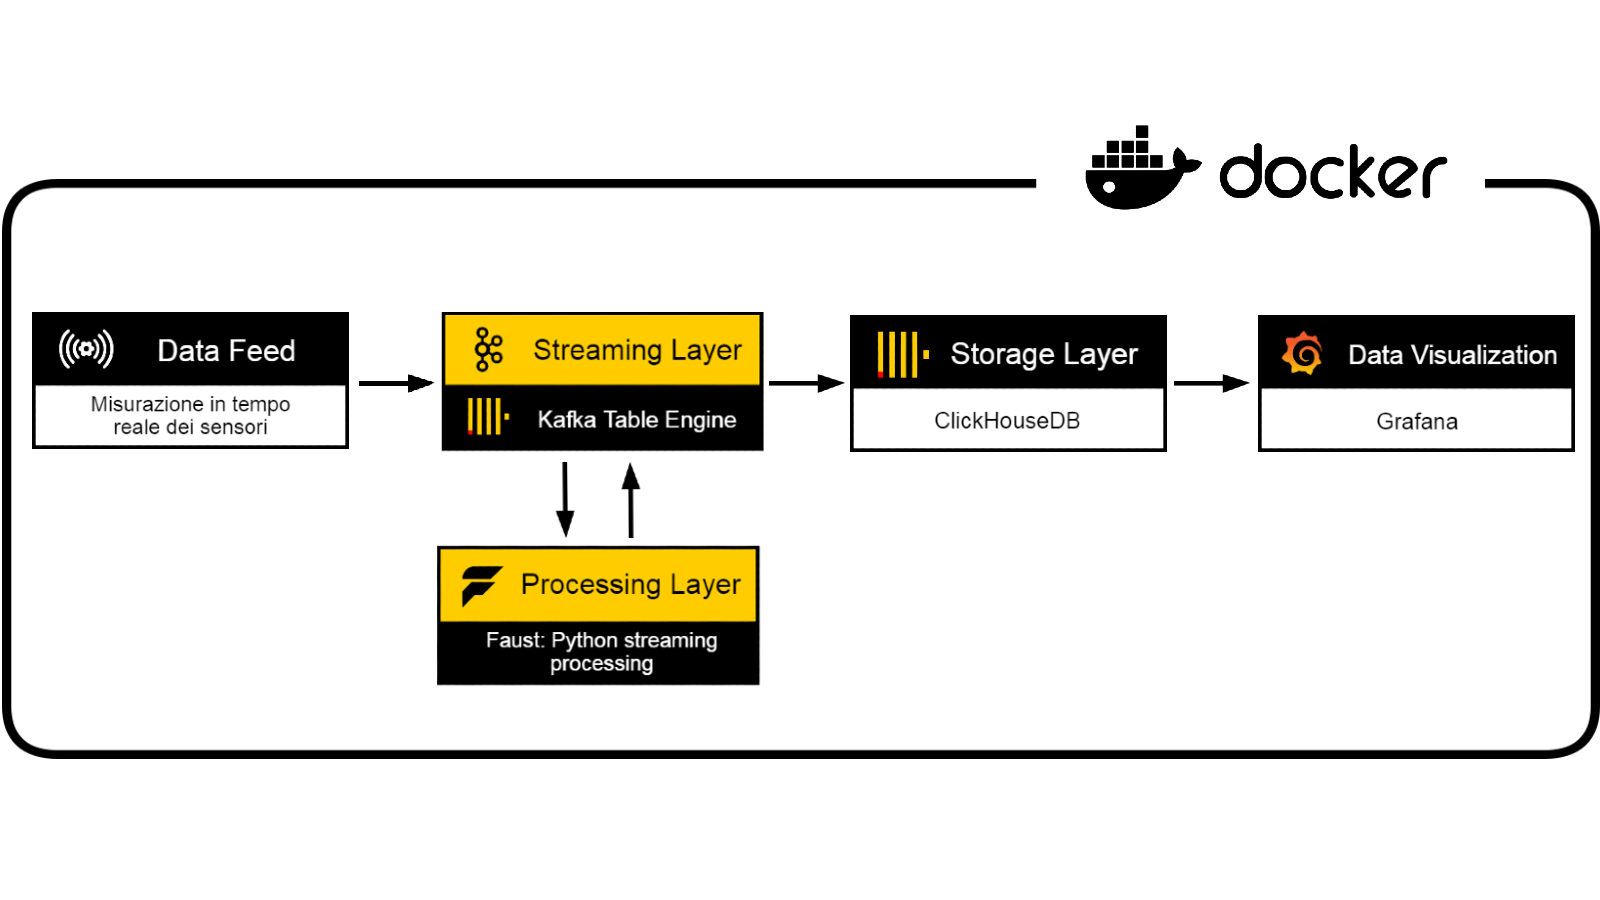
\includegraphics[width=1\textwidth]{../Images/SpecificaTecnica/architettura.jpg}
    \caption{Componenti dell'architettura - innovacity}
    \label{fig: fdf}
\end{figure}

\begin{itemize}
    \item \textbf{Data feed}:Le sorgenti dati sono costituite da sensori IoT dislocati sul territorio cittadino. Questi sensori sono in grado di inviare, ad intervalli regolari, messaggi contenenti misurazioni allo streaming layer;
    \item \textbf{Streaming layer}:Lo streaming layer gestisce i dati in arrivo in tempo reale, per poi archiviarli sistematicamente nello storage layer. Lo streaming Layer è composto da:
    \begin{itemize}
        \item \textbf{Apache Kafka}: Kafka è un sistema di messaggistica distribuito che consente di pubblicare, sottoscrivere e archiviare messaggi in tempo reale. Kafka è utilizzato per ricevere i dati dai sensori IoT e renderli disponibili per l'elaborazione in tempo reale e batch.
        \item \textbf{Clickhouse Kafka table engine}:consumatore che legge i
        dati dal server Kafka per persisterli nello storage layer.
    \end{itemize}
    \item \textbf{Processing Layer:} Il processing Layer è costituito da Faust che consuma i dati dallo streaming layer e li processa in tempo reale. Faust è un framework Python che consente di scrivere applicazioni di streaming in tempo reale. Faust è utilizzato per elaborare i dati in arrivo tramite un modello per il calcolo del punteggio di salute che poi viene reso nuovamente disponibili allo streaming layer.
    \item \textbf{Storage layer}:Lo storage layer è costituito da un database column-oriented, ClickHouse, che archivia i dati in arrivo dallo streaming layer. Questi dati sono disponibili per l'analisi e la visualizzazione in tempo reale e batch.
    \item \textbf{Data Visualization Layer}: composto da Grafana, si occupa della visualizzazione dei dati elaborati ottenuti dallo storage layer e della gestione delle notifiche in caso di anomalie rilevate.
\end{itemize}
\subsection{Architettura dei simulatori} \label{sec:architettura_simulatori}
Nonostante i simulatori non siano ufficialmente considerati parte integrante del prodotto dalla proponente, il nostro team ha scelto di dedicare alcune risorse alla progettazione di questa componente nell'ambito del progetto didattico. Inoltre, abbiamo deciso di implementare e tenere conto delle possibili logiche dei microcontrollori associati ai sensori IoT, che possono effettuare operazioni per rendere più efficiente l'intero sistema.

Nei paragrafi successivi, verrà presentata l'architettura individuata mediante l'utilizzo di diagrammi delle classi e relative descrizioni rapide. Inoltre, saranno motivate le scelte dei design pattern individuati e le decisioni progettuali rilevanti. Successivamente, per ogni classe, saranno illustrati metodi e attributi.
\subsubsection{Modulo simulatori sensori}
\begin{figure}[H]
    \centering
    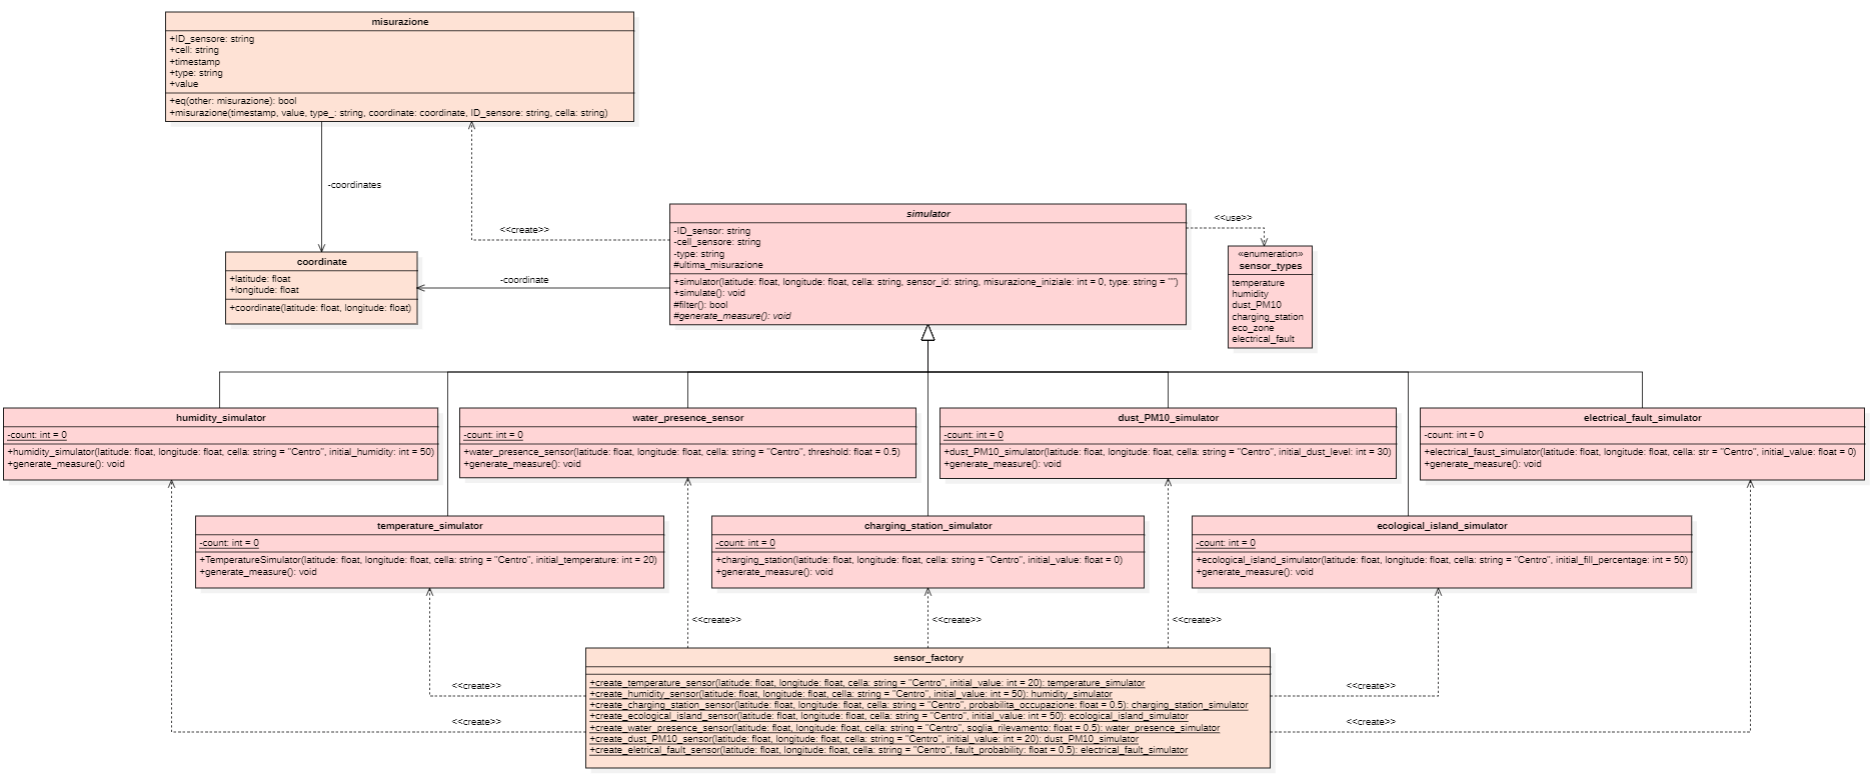
\includegraphics[width=1\textwidth]{../Images/SpecificaTecnica/simulatoriSensori.PNG}
    \caption{Modulo simulatori sensori - innovacity}
    \label{fig: fddf}
\end{figure}
Questo modulo si occupa della generazione di dati di misurazione per diverse tipologie di sensori.

\paragraph{Design pattern Template Method:}

La classe astratta \textit{Simulator} implementa il design pattern \textit{Template Method}. Il metodo \textit{simulate()} fornisce lo scheletro dell'algoritmo per la generazione e la gestione delle misurazioni. Le classi concrete che estendono \textit{Simulator} implementano:
\begin{itemize}
    \item \textbf{Metodo \textit{generate\_measure()}}: per la generazione semi randomica della misurazione associata al tipo di sensore;
    \item \textbf{Metodo \textit{filter()}}: per la logica di filtrazione di misurazioni errate o non attendibili (ad esempio, negative, fuori range o consecutive troppo distanti). Il metodo \textit{filter()} offre un'implementazione di default che lascia passare ogni misurazione senza modifiche.
\end{itemize}

Il design pattern \textit{Template Method} è stato scelto per:
\begin{itemize}
    \item Permettere una facile estensione del sistema con nuovi tipi di sensori che dovranno unicamente implementare la loro logica di generazione delle misurazioni e di filtering se necessario;
    \item Standardizzare i passi per la generazione delle misurazioni, garantendo coerenza e manutenibilità del codice;
    \item Ridurre la duplicazione del codice.
\end{itemize}

Una volta ottenuto lo stato del sensore, esso viene inserito in un oggetto di tipo \textit{Misurazione}. Questo oggetto contiene informazioni di contesto come:
\begin{itemize}
    \item Identificativo del sensore;
    \item Cella della città in cui è presente;
    \item Timestamp della misurazione;
    \item Valore della misurazione;
    \item Coordinate;
    \item Tipologia di misurazione.
\end{itemize}
L'oggetto \textit{Misurazione} viene poi ritornato al chiamante che si occuperà di inviarlo al server \textit{Kafka}.
Un oggetto di tipo \textit{Simulator} verrà assegnato ad ogni \textit{SimulatorThread} che chiamerà ad intervalli regolari il metodo \textit{simulate()} ottenendo appunto la misurazione che invierà al server \textit{Kafka} tramite un modulo apposito e indipendendente.

\paragraph{Design pattern Factory:}
SensorFactory implementa il design pattern \textit{Factory} per la creazione di simulatori dei sensori.
Il pattern FACTORY è un pattern di tipo “Creazionale” secondo la classificazione della GoF.
I pattern di tipo creazionali si occupano della costruzione delle simulazioni dei sensori e delle problematiche che si possono originare, astraggono il processo di creazione degli oggetti, nascondono i dettagli della creazione e rendono i sistemi indipendenti da come gli oggetti sono creati e composti.
Il pattern Factory incapsula la creazione concreta dei sensori, consentendo al client
(l’utilizzatore) di non conoscere i dettagli.


\paragraph{Classi: metodi e attributi}
\begin{itemize}
    \item {\textbf{Classe astratta: \textit{Simulator}}}
        \begin{itemize}
            \item \textbf{Attributi}: 
            \begin{itemize}
                \item \textbf{ID\_sensor:str [private]} - Identificatore univoco del sensore.
                \item \textbf{cella\_sensore:str [private]} - Identificatore della cella del sensore.
                \item \textbf{coordinate:Coordinate [private]} - Coordinate geografiche del sensore.
                \item \textbf{misurazione: T [protected]} - Misurazione corrente del sensore.
                \item \textbf{type:str [private]} - Tipo di sensore.
            \end{itemize}
            \item \textbf{Metodi}:
            \begin{itemize}
                \item \textbf{simulate():Misurazione [public]} - Metodo principale per simulare la generazione di una misurazione.
                Si basa sul design pattern Template Method:
                \begin{enumerate}
                    \item     Chiama generate\_measure() per generare un valore di misurazione.
                    \item     Verifica con filter() se la misurazione è valida (ripete la generazione finché non lo è).
                    \item     Restituisce un oggetto Misurazione con data e ora corrente, valore misurato, tipo di sensore, coordinate e identificativo del sensore.
                \end{enumerate}
                \item \textbf{generate\_measure():None [protected]} - Metodo astratto da implementare nelle classi concrete per generare un valore di misurazione semi-casuale coerente con la tipolgia di sensore da salvare nell'attributo \textit{misurazione}.
                \item \textbf{filter():bool [protected]} - Metodo di filtro per la validazione della misurazione (implementazione di default che accetta sempre la misurazione). Può essere ridefinito nelle classi concrete per implementare la logica di filtraggio.
            \end{itemize}
            \item \textbf{Note}:
            \begin{itemize}
                \item La classe Simulator è astratta e definisce il comportamento generale della simulazione della misurazione.
                \item Le classi concrete che ereditano da Simulator devono implementare il metodo astratto generate\_measure().
                \item Il metodo filter() può essere ridefinito nelle classi concrete per implementare la logica di validazione specifica del sensore.
            \end{itemize}
        \end{itemize}
        
        
        
        
        \item{\textbf{Enumerazione: \textit{SensorTypes}}}
        \begin{itemize}
            \item \textbf{Costanti}: 
            \begin{itemize}
                \item \textbf{TEMPERATURE:str [public]} - Rappresenta la nomenclatura dei sensore di temperatura.
                \item \textbf{HUMIDITY:str [public]} - Rappresenta la nomenclatura dei sensore di umidità.
                \item \textbf{DUST\_PM10:str [public]} - Rappresenta la nomenclatura dei sensore di "polvere PM10".
                \item \textbf{CHARGING\_STATION:str [public]} - Rappresenta la nomenclatura dei sensore di stato delle colonnine di ricarica.
                \item \textbf{ECOLOGICAL\_ISLAND:str [public]} - Rappresenta la nomenclatura dei sensore di stato riempimento isole ecologica.
                \item \textbf{WATER\_PRESENCE:str [public]} - Rappresenta la nomenclatura dei sensore di presenza d'acqua.
                \item \textbf{ELECTRICAL\_FAULT:str [public]} - Rappresenta la nomenclatura dei sensore di guasti elettrici.
            \end{itemize}

            \item \textbf{Note}:
            \begin{itemize}
                \item L'enumerazione viene utilizzata per centralizzare la gestione della nomenclatura dei tipi di sensori che verrà salvata nelle misurazioni.
            \end{itemize}
        \end{itemize}
        
        
    \item{\textbf{Classe: \textit{TemperatureSimulator}}}
    \begin{itemize}
        \item \textbf{Attributi:}
    \begin{itemize}
        \item \textbf{count:int [private, static]} - Contatore statico per generare un ID univoco per ogni istanza.
    \end{itemize}
    \item\textbf{Metodi}: 
    \begin{itemize}
        \item \textbf{generate\_measure():None [protected]} - Genera una misurazione di temperatura semi-casuale e aggiorna la misurazione corrente.
    \end{itemize}
    \item\textbf{Note}:
    \begin{itemize}
        \item La classe TemperatureSimulator è una classe concreta che eredita dalla classe astratta Simulator.
        \item Il costruttore genera automaticamente un ID sensore univoco per ogni istanza.
    \end{itemize}
\end{itemize}
    \item{\textbf{Classe: \textit{HumiditySimulator}}}
    \begin{itemize}
        \item\textbf{Attributi:}
    \begin{itemize}
        \item \textbf{count:int [private, static]} - Contatore statico per generare un ID univoco per ogni istanza.
    \end{itemize}
    \item \textbf{Metodi}: 
    \begin{itemize}
        \item \textbf{generate\_measure():None [protected]} - Genera una misurazione di umidità semi-casuale e aggiorna la misurazione corrente.
    \end{itemize}
    \item \textbf{Note}:
    \begin{itemize}
        \item La classe HumiditySimulator è una classe concreta che eredita dalla classe astratta Simulator.
        \item Il costruttore genera automaticamente un ID sensore univoco per ogni istanza.
    \end{itemize}
\end{itemize}
    \item{\textbf{Classe: \textit{ChargingStationSimulator}}}
    \begin{itemize}
        \item  \textbf{Attributi}: 
    \begin{itemize}
        \item \textbf{count:int [private, static]} - Contatore statico per generare un ID univoco per ogni istanza.
    \end{itemize}
    \item  \textbf{Metodi}:
    \begin{itemize}
        \item \textbf{generate\_measure():None [protected]} - Genera lo stato della colonnina di ricarica (Occupato: True, Libero: False) basata su una probabilità di transizione.
    \end{itemize}
    \item   \textbf{Note}:
    \begin{itemize}
        \item La classe ChargingStationSimulator è una classe concreta che eredita dalla classe astratta Simulator.
        \item Implementa il metodo astratto generate\_measure() per generare una misurazione basata sulla probabilità di transizione.
        \item Il costruttore genera automaticamente un ID sensore univoco per ogni istanza.
    \end{itemize}
\end{itemize}
    \item{\textbf{Classe: \textit{DustPM10Simulator}}}
    \begin{itemize}
        \item   \textbf{Attributi}: 
    \begin{itemize}
        \item \textbf{count:int [private, static]} - Contatore statico per generare un ID univoco per ogni istanza.
    \end{itemize}
    \item    \textbf{Metodi}: 
    \begin{itemize}
        \item \textbf{generate\_measure():None [protected]} - Genera una variazione di polvere PM10 semi-casuale e aggiorna la misurazione corrente.
    \end{itemize}
    \item    \textbf{Note}:
    \begin{itemize}
        \item La classe DustPM10Simulator è una classe concreta che eredita dalla classe astratta Simulator.
        \item Il costruttore genera automaticamente un ID sensore univoco per ogni istanza.
    \end{itemize}
\end{itemize}
    \item{\textbf{Classe: \textit{ElectricalFaultSimulator}}}
    \begin{itemize}
        \item   \textbf{Attributi}: 
    \begin{itemize}
        \item \textbf{count:int [private, static]} - Contatore statico per generare un ID univoco per ogni istanza.
    \end{itemize}
    \item   \textbf{Metodi}: 
    \begin{itemize}
        \item \textbf{generate\_measure():None [protected]} - Genera lo stato di una centralina elettrica (Guasto verificato: True, Operativa: False) basata sulla probabilità di guasto.
    \end{itemize}
    \item   \textbf{Note}:
    \begin{itemize}
        \item La classe ElectricalFaultSimulator è una classe concreta che eredita dalla classe astratta Simulator.
        \item Il costruttore genera automaticamente un ID sensore univoco per ogni istanza.
    \end{itemize}
\end{itemize}
    \item{\textbf{Classe: \textit{EcologicalIslandSimulator}}}
    \begin{itemize}
        \item    \textbf{Attributi}: 
    \begin{itemize}
        \item \textbf{count:int [private, static]} - Contatore statico per generare un ID univoco per ogni istanza.
    \end{itemize}
    \item    \textbf{Metodi}: 
    \begin{itemize}
        \item \textbf{generate\_measure():None [protected]} - Genera una misurazione della percentuale di riempimento di un isola ecologica.
    \end{itemize}
    \item    \textbf{Note}:
    \begin{itemize}
        \item La classe EcologicalIslandSimulator è una classe concreta che eredita dalla classe astratta Simulator.
        \item Il costruttore genera automaticamente un ID sensore univoco per ogni istanza.
    \end{itemize}
\end{itemize}
    \item{\textbf{Classe: \textit{WaterPresenceSensor}}}
    \begin{itemize}
        \item    \textbf{Attributi}: 
    \begin{itemize}
        \item \textbf{count:int [private, static]} - Contatore statico per generare un ID univoco per ogni istanza.
    \end{itemize}
    \item    \textbf{Metodi}: 
    \begin{itemize}
        \item \textbf{generate\_measure():None [protected]} - Genera una misurazione basata sulla soglia di presenza dell'acqua (Acqua rilevata: True, Acqua non rilevata:False).
    \end{itemize}
    \item    \textbf{Note}:
    \begin{itemize}
        \item La classe EcologicalIslandSimulator è una classe concreta che eredita dalla classe astratta Simulator.
        \item Il costruttore genera automaticamente un ID sensore univoco per ogni istanza.
    \end{itemize}
\end{itemize}
    \item{\textbf{Classe: \textit{Misurazione}}}
    \begin{itemize}
        \item   \textbf{Attributi}: 
    \begin{itemize}
        \item \textbf{timestamp:datetime [private]} - Timestamp della misurazione.
        \item \textbf{value:T [private]} - Valore della misurazione.
        \item \textbf{type:str [private]} - Tipo della misurazione.
        \item \textbf{coordinates:Coordinate [private]} - Coordinate della misurazione.
        \item \textbf{ID\_sensore:str [private]} - ID del sensore che ha effettuato la misurazione.
        \item \textbf{cella:str [private]} - Cella in cui è stata effettuata la misurazione.
    \end{itemize}
    \item   \textbf{Metodi}: 
    \begin{itemize}
        \item \textbf{\_\_eq\_\_(other:Misurazione):bool [public]} - Ridefinizione dell'operatore di uguaglianza per confrontare due oggetti Misurazione.
    \end{itemize}
\end{itemize}
    \item{\textbf{Classe: \textit{Coordinate}}}
    \begin{itemize}
        \item    \textbf{Attributi}: 
    \begin{itemize}
        \item \textbf{latitude:float [private]} - Latitudine della coordinata.
        \item \textbf{longitude:float [private]} - Longitudine della coordinata.
    \end{itemize}
    \item     \textbf{Metodi}: 
    \begin{itemize}
        \item \textbf{\_\_eq\_\_(other:Coordinate):bool [public]} - Ridefinizione dell'operatore di uguaglianza per confrontare due oggetti Coordinate.
    \end{itemize}
\end{itemize}
    \item{\textbf{Classe: \textit{SensorFactory}}}
    \begin{itemize}
        \item    \textbf{Metodi}: 
\begin{itemize}
    \item \textbf{create\_temperature\_sensor(latitude: float, longitude: float, cella: str, initial\_value:float):TemperatureSimulator [public, static]} - Crea un simulatore di temperatura.
    \item \textbf{create\_humidity\_sensor(latitude: float, longitude: float, cella: str, initial\_value:float):HumiditySimulator [public, static]} - Crea un simulatore di umidità.
    \item \textbf{create\_charging\_station\_sensor(latitude: float, longitude: float, cella: str, probabilita\_occupazione:float):ChargingStationSimulator [public, static]} - Crea un simulatore di stazione di ricarica.
    \item \textbf{create\_ecological\_island\_sensor(latitude: float, longitude: float, cella: str, initial\_value:float):EcologicalIslandSimulator [public, static]} - Crea un simulatore di isola ecologica.
    \item \textbf{create\_water\_presence\_sensor(latitude: float, longitude: float, cella: str, soglia\_rilevamento:float):WaterPresenceSensor [public, static]} - Crea un sensore di presenza d'acqua.
    \item \textbf{create\_dust\_PM10\_sensor(latitude: float, longitude: float, cella: str, initial\_value:float):DustPM10Simulator [public, static]} - Crea un simulatore di polvere PM10.
    \item \textbf{create\_eletrical\_fault\_sensor(latitude: float, longitude: float, cella: str, fault\_probability:float):ElectricalFaultSimulator [public, static]} - Crea un simulatore di guasto elettrico.
\end{itemize}
\textbf{Note}:
    \begin{itemize}
        \item Implementazione del Pattern Factory;
        \item Fornisce metodi per la creazione di simulatori di sensori;
        \item Astrae il processo di creazione dei sensori, nascondendo i dettagli della creazione.
    \end{itemize}
\end{itemize}
\end{itemize}




\subsubsection{Modulo Writers}
\begin{figure}[H]
    \centering
    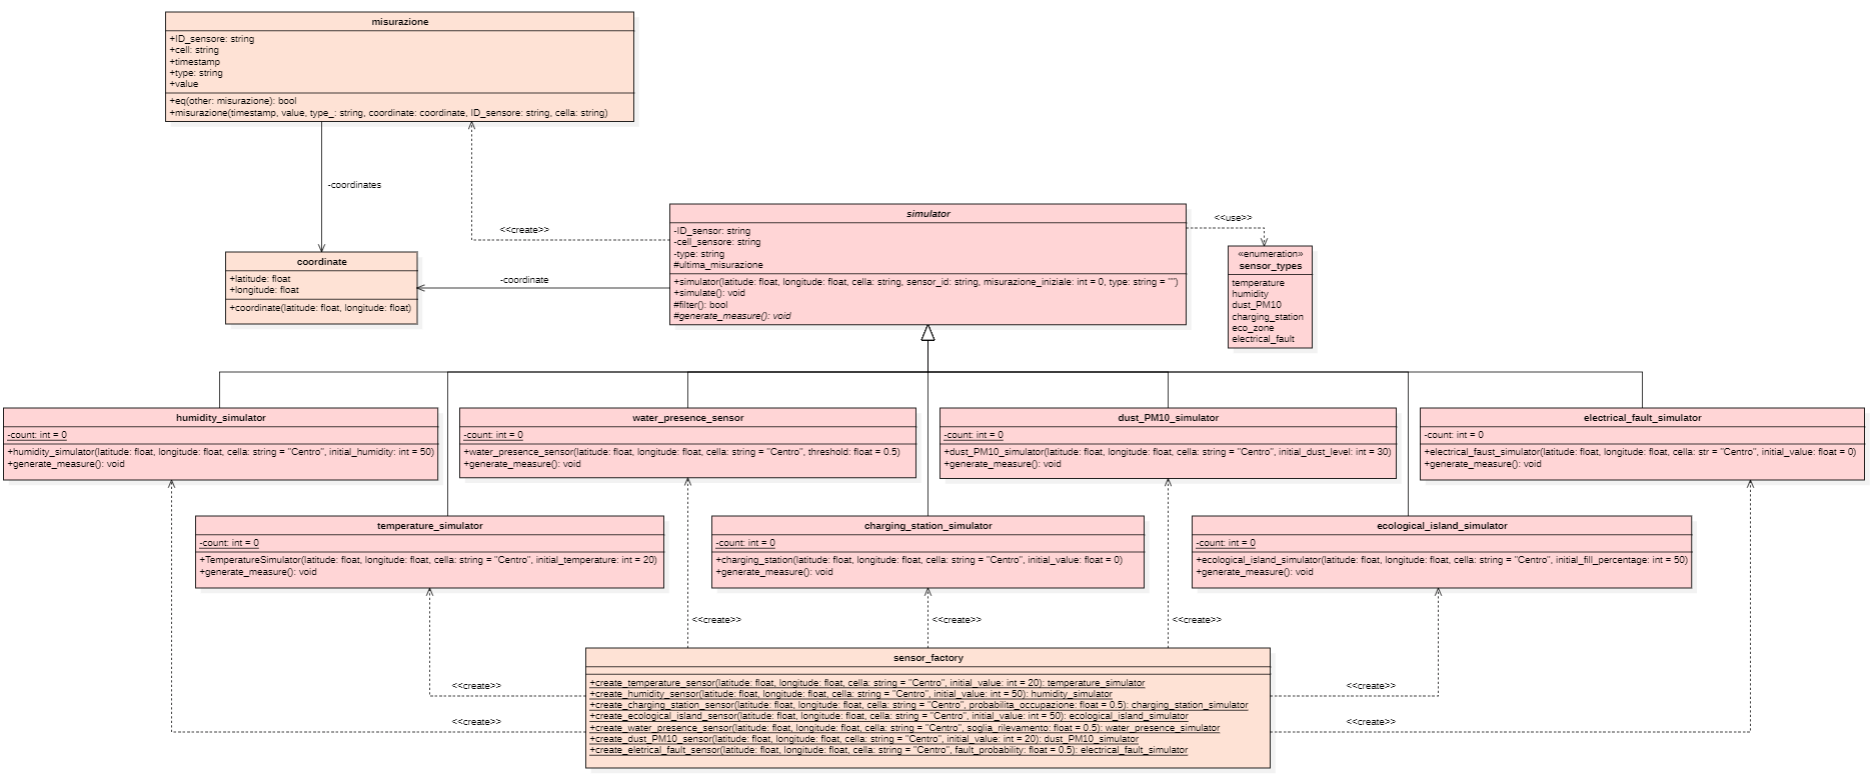
\includegraphics[width=1\textwidth]{../Images/SpecificaTecnica/simulatoriSensori.PNG}
    \caption{Modulo writers - innovacity}
    \label{fig: fdsd}
\end{figure}

Questo modulo si occupa della scrittura e/o invio di informazioni a diverse tipologie di servizi e vuole essere completamentemente indipendendente e non influenzato dal modulo della simulazione dei sensori cosi da poter consentire un suo riutilizzo.

\paragraph{Design pattern Strategy + Composite:}
Il modulo presenta un interfaccia \textit{Writer} che offre il metodo di scrittura \textit{write()} di oggetti di tipo \textit{Writable}.
Questo metodo è implementato da diverse classi concrete che rappresentano i vari servizi a cui è possibile inviare le informazioni.
Questo approccio implementa il design pattern \textit{Strategy} per la scrittura dei dati su diverse piattaforme/servizi e il design pattern \textit{Composite} per la gestione di più servizi a cui scrivere contemporaneamente in modo completamentemente indifferenziato dalla scrittura ad un singolo servizio.
Nello specifico sono state implentate tre strategie di scrittura:la prima, (\textit{KafkaWriter}), atta a permettere al simulatore di inviare messaggi a Kafka,  la seconda (\textit{StdOutWriter}) atta a permettere di stampare i \textit{Writable}su terminale e la terza (\textit{ListWriter}) per il salvataggio su una lista degli oggetti \textit{Writable}.
L'utilizzo del design pattern Composite e Strategy in questo caso ha diverse motivazioni:
\begin{itemize}
    \item \textbf{Gestione uniforme dei servizi}: Il pattern Strategy consente di definire una famiglia di algoritmi, incapsularli e renderli intercambiabili. In questo caso, i servizi di scrittura sono trattati come algoritmi intercambiabili, consentendo di scrivere informazioni su diversi servizi senza dover conoscere i dettagli di implementazione di ciascuno.
    \item \textbf{Gestione gerarchica dei servizi}: Il pattern Composite consente di trattare gli oggetti singoli e le loro composizioni (gruppi di oggetti) allo stesso modo. Nel contesto del modulo, potrebbe esserci la necessità di gestire non solo singoli servizi, ma anche gruppi di servizi. Ad esempio, potrebbe essere utile inviare informazioni contemporaneamente a diversi servizi, come un database, un file di log e un servizio di notifica. Il Composite consente di comporre questi servizi in modo gerarchico e trattarli uniformemente.
\end{itemize}

\paragraph{Design pattern Object Adapter:}
Nello specifico, la classe \textit{KafkaWriter} realizza la sua funzionalità attraverso l'utilizzo del design pattern \textit{Adapter}, nella sua variante \textit{Object Adapter}. Tale scelta è stata motivata dall'impiego della classe \textit{Producer} della libreria \textit{confluent\_kafka}, la quale potrebbe subire variazioni non controllabili da noi. Per garantire la capacità di rispondere prontamente a tali cambiamenti senza dover modificare la classe \textit{KafkaWriter} o altri parti di sistema, si è optato per l'utilizzo di questo pattern, trasferendo così la complessità derivante da tali modifiche proprio nell'adapter.
Inoltre grazie all'interfaccia \textit{KafkaTarget}, si è garantita la possibilità di estendere il sistema con nuovi metodi di scrittura su Kafka o l'utilizzo di nuove librerie senza dover modificare la classe \textit{KafkaWriter} ma solamente aggiungendo una nuova classe adapter che implementi \textit{KafkaTarget}.



\paragraph{Classi: metodi e attributi}

\begin{itemize}
    \item{\textbf{Interfaccia: \textit{Writable}}}
    \begin{itemize}
        \item\textbf{Metodi}: 
        \begin{itemize}
            \item \textbf{to\_json(): [public, abstract]} - Metodo astratto che deve essere implementato nelle sottoclassi per convertire l'oggetto in una stringa JSON.
        \end{itemize}
        \item\textbf{Note}:
        \begin{itemize}
            \item L'interfaccia \textit{Writable} definisce un insieme di metodi che una classe deve implementare perchè possa essere utilizzata dalle strategie di scrittura.
        \end{itemize}
    \end{itemize}
    \item{\textbf{Interfaccia: \textit{Writer}}}
     \begin{itemize}
        \item \textbf{Metodi:}
         \begin{itemize}
            \item \textbf{write(to\_write: Writable): None [public, abstract]} - Metodo astratto che deve essere implementato nelle sottoclassi per scrivere un oggetto Writable.
        \end{itemize}
        \item\textbf{Note}:
        \begin{itemize}
            \item L'interfaccia \textit{Writer} definisce un insieme di metodi che una classe deve implementare perchè possa essere utilizzata come strategia di scrittura;
            \item Rappresenta l'interfaccia "Component" del pattern \textit{Composite} che descrive le operazioni comuni sia agli elementi semplici che a quelli complessi dell'albero.
        \end{itemize}
    \end{itemize}
    \item{\textbf{Classe: \textit{StdoutWriter}}}
    \begin{itemize}
    \item\textbf{Attributi}:
        \begin{itemize}
        \item \textbf{lock:threading.Lock [private]} - Lock per garantire l'accesso esclusivo alla stampa ed un esecuzione Thread safe.
    \end{itemize}
    \item \textbf{Metodi: }
    \begin{itemize}
        \item \textbf{write(to\_write: Writable): None [public]} - Stampa l'oggetto Writable come stringa JSON nella console;
    \end{itemize}
    \item\textbf{Note}:
        \begin{itemize}
            \item La classe è una strategia di scrittura del pattern \textit{Strategy} ma anche la componente "Leaf" del pattern \textit{Composite}, ovvero l'elemento base che non ha sottoelementi.
        \end{itemize}
    \end{itemize}
    \item{\textbf{Classe: \textit{ListWriter}}}
    \begin{itemize}
    \item\textbf{Attributi}:
        \begin{itemize}
        \item \textbf{data\_list:list [private]} - Lista per memorizzare gli oggetti Writable.
        \item \textbf{lock:threading.Lock [private]} - Lock per garantire l'accesso esclusivo alla lista ed un esecuzione Thread safe.
    \end{itemize}
    \item \textbf{Metodi: }
    \begin{itemize}
        \item \textbf{write(to\_write: Writable): None [public]} - Aggiunge l'oggetto Writable alla lista.
        \item \textbf{get\_data\_list(): list [public]} - Restituisce la lista di oggetti Writable.
    \end{itemize}
    \item\textbf{Note}:
        \begin{itemize}
            \item La classe è una strategia di scrittura del pattern \textit{Strategy} ma anche la componente "Leaf" del pattern \textit{Composite}, ovvero l'elemento base che non ha sottoelementi.
        \end{itemize}
    \end{itemize}
    \item{\textbf{Classe: \textit{KafkaWriter}}}
    \begin{itemize}
    \item\textbf{Attributi}:
        \begin{itemize}
        \item \textbf{lock:threading.Lock [private]} - Lock per garantire l'accesso esclusivo alla scrittura su Kafka ed un esecuzione Thread safe.
        \item \textbf{kafka\_target:KafkaTarget [private]} - Riferimento ad un implementazione di KafkaTarget per effettuare l'effettiva scrittura in Kafka tramite librerie.
    \end{itemize}
    \item \textbf{Metodi: }
    \begin{itemize}
        \item \textbf{write(to\_write: Writable): None [public]} - Scrive l'oggetto Writable come stringa JSON su Kafka.
    \end{itemize}
    \item\textbf{Note}:
        \begin{itemize}
            \item La classe è una strategia di scrittura del pattern \textit{Strategy} ma anche la componente "Leaf" del pattern \textit{Composite}, ovvero l'elemento base che non ha sottoelementi.
            \item La costruzione dell'oggetto KafkaWriter richiede un riferimento ad un oggetto che implementi l'interfaccia KafkaTarget.
        \end{itemize}
    \end{itemize}
    \item{\textbf{Classe: \textit{CompositeWriter}}}
    \begin{itemize}
    \item\textbf{Attributi}:
        \begin{itemize}
        \item \textbf{writers:Writer* [protected]} - Lista di oggetti Writer.
    \end{itemize}
    \item \textbf{Metodi: }
    \begin{itemize}
        \item \textbf{add\_writer(writer: Writer): CompositeWriter [public]} - Aggiunge un oggetto Writer alla lista di writers.
        \item \textbf{add\_kafkaConfluent\_writer(topic: str, host: str, port: int): CompositeWriter [public]} - Crea un KafkaWriter con un KafkaConfluentAdapter e lo aggiunge alla lista di writers.
        \item \textbf{add\_stdOut\_writer(): CompositeWriter [public]} - Crea un StdoutWriter e lo aggiunge alla lista di writers.
        \item \textbf{add\_list\_writer(writer\_list: ListWriter): CompositeWriter [public]} - Aggiunge un ListWriter alla lista di writers.
        \item \textbf{remove\_writer(writer: Writer): None [public]} - Rimuove un Writer dalla lista di writers.
        \item \textbf{write(to\_write: Writable): None [public]} - Chiama il metodo write su ogni Writer nella lista di writers passando come attributo il \textit{Writable} ricevuto.
    \end{itemize}
    \item\textbf{Note}:
        \begin{itemize}
            \item La classe è la componente "Composite" del pattern \textit{Composite}, ovvero l'elemento che può avere sottoelementi;
            \item Dopo aver ricevuto una richiesta, il contenitore (detto compisite) delega il lavoro ai suoi sottoelementi:foglie o altri contenitori.
        \end{itemize}
    \end{itemize}
    \item{\textbf{Interfaccia: \textit{KafkaTarget}}}
    \begin{itemize}
    \item \textbf{Metodi: }
    \begin{itemize}
        \item \textbf{write\_to\_kafka(data: str): None [public, abstract]} - Metodo astratto che deve essere implementato nelle sottoclassi per scrivere dati su Kafka.
    \end{itemize}
    \item\textbf{Note}:
        \begin{itemize}
            \item La classe è una interfaccia che fornisce un contratto per le operazioni di scrittura e invio a Kafka.
            \item Rappresenta il componente Target del pattern \textit{Object Adapter}.
        \end{itemize}
    \end{itemize}
\end{itemize}
\subsubsection{Modulo Threading/Scheduling}


\paragraph{Classi: metodi e attributi}




\subsection{Kafka}
\subsubsection{Kafka topic}
I topic in Kafka possono essere considerati come le tabelle di un database, utili per separare logicamente diversi tipi di messaggi o eventi che vengono inseriti nel sistema. Noi li utilizziamo per separare le diverse misurazioni dei sensori, quindi per ogni tipo di sensore è presente un topic dedicato. Ciò ci consente di creare all'interno di ClickHouse delle "tabelle consumatrici" che acquisiscono automaticamente i dati. Questo è possibile grazie alla separazione logica dei topic, che garantisce che tutti i messaggi all'interno di ciascun topic abbiano lo stesso formato.
\subsection{Formato messaggi} \label{sec:formatoMessaggi}
La struttura di un messaggio contenente le informazioni della misurazione è la seguente in formato Json:
\begin{comment}
    \begin{lstlisting}[language=json,firstnumber=1]
    {
      "timestamp": "AAAA-MM-DD HH:MM:SS.sss", 
      "value": "Valore della misurazione",  
      "type": "Tipologia Simulatore",
      "latitude": "Latitudine",
      "longitude": "Longitudine",
      "ID_sensore": "ID sensore",
      "cella": "Cella dove è presente il sensore"
    }
\end{lstlisting}
\end{comment}


Sebbene le misurazioni vengano divise in topic diversi a seconda della tipoligia di sensore che ha effettuato la misurazione si è comunque deciso di inviare e salvare il campo della tipoligia di misurazione per i seguenti motivi:
\begin{itemize}
    \item \textbf{Backup e ripristino dei dati:} Se per qualche motivo si dovesse perdere la struttura dei topic o occorre ripristinare i dati in un altro sistema, il campo type può aiutare a identificare il tipo di sensore che ha effettuato la misurazione, anche se i dati sono stati conservati insieme in un unico topic.
    \item \textbf{Flessibilità futura:} 
    \begin{itemize}
        \item Potrebbero sorgere esigenze future che richiedono l'analisi dei dati provenienti da diversi tipi di sensori all'interno dello stesso topic. In questo caso, il campo type sarebbe utile per distinguere le misurazioni provenienti da sensori diversi;
        \item includere il campo type potrebbe essere particolarmente utile se si prevede di supportare diverse unità di misura per una stessa tipologia di sensore in futuro. Ad esempio, potrebbe essere necessario gestire misurazioni di temperatura in gradi Celsius, Fahrenheit o Kelvin. In tal caso, includendo il campo type, si può associare ad ogni misurazione l'unità di misura corretta.
    \end{itemize}
\end{itemize}
    
\subsection{Faust - Processing Layer} \label{sec:faust}
\subsubsection{Introduzione}
\paragraph*{Premessa}

Per soddisfare il requisito opzionale del calcolo del punteggio di salute, si è scelto di utilizzare Faust, una libreria Python ispirata al modello di Kafka Streams. Faust facilita l'elaborazione di flussi di dati distribuiti in tempo reale, rendendola ideale per questo caso d'uso.
Offre un'interfaccia di alto livello che astrae le complessità di Kafka, rendendo la raccolta dati semplice e intuitiva.
Inolltre Faust è progettato per essere scalabile e può essere utilizzato per gestire grandi volumi di dati.

\paragraph*{Calcolo del Punteggio}
Il punteggio di salute rappresenta un indicatore sintetico del benessere generale di una città, misurandolo in base a diversi aspetti chiave. In questo caso, le tre tipologie di misurazioni considerate sono:
\begin{itemize}
    \item Temperatura;
    \item Umidità;
    \item Livello di polveri sottili (PM10).
\end{itemize}

Il calcolo del punteggio avviene in due fasi:
\begin{enumerate}
    \item \textbf{Incrementi}: 
    \begin{itemize}
        \item A intervalli regolari, si calcolano incrementi al punteggio di salute basandosi sulle misurazioni acquisite nell'intervallo precedente.
        \item Ciascuna tipologia di misurazione ha un suo algoritmo di calcolo dell'incremento, basato su soglie predefinite di benessere.
    \end{itemize}
    \item \textbf{Punteggio Finale}:
    \begin{itemize}
        \item Il punteggio di salute finale si ottiene sommando gli incrementi calcolati per le tre tipologie di misurazioni.
        \item Punteggi più alti indicano un minore stato di benessere, con la necessità di interventi per migliorare la qualità della vita.
    \end{itemize}
\end{enumerate}


\subsubsection{Componenti Faust \& Processing Layer}
\begin{itemize}
    \item \textbf{Applicazione Faust:}
    \begin{lstlisting}[style=code]
        faust.App(<nome_app>, broker=<broker_kafka>)
    \end{lstlisting} 
    \begin{itemize}
        \item Un'applicazione Faust è un programma Python che elabora flussi di dati in tempo reale da Kafka.
        \item \textbf{nome\_app}: Identifica l'applicazione.
        \item \textbf{broker\_kafka}: Indirizzo del broker Kafka (hostname:porta).
    \end{itemize}
    \item \textbf{Topic:}
    \begin{lstlisting}[style=code]
        app.topic(<nome_topic>, value_type=<tipo_dato>)
    \end{lstlisting}  
    \begin{itemize}
        \item \textbf{nome\_topic}: Nome del topic Kafka.
        \item \textbf{tipo\_dato:} Classe che rappresenta il tipo di dato del topic (es. FaustMeasurement).
        \item Nel caso si voglia aggiungere altri topic da cui consumare dati basterà aggiungerne prima del parametro value\_type.
    \end{itemize}
    \item \textbf{Tipo di dato atteso:}
     \begin{lstlisting}[style=code]
        class FaustMeasurement(faust.Record)
    \end{lstlisting}  
    \begin{itemize}
        \item È una classe che eredita da \textbf{faust.Record}.
        \item \textbf{faust.Record} è una classe fornita dalla libreria Faust che semplifica la definizione di record per la rappresentazione dei dati in streaming.
        \item Rappresenta una singola misurazione proveniente da un sensore. Viene usata nella applicazione Faust per definire il tipo di dati atteso nei topic Kafka.
    \end{itemize}
    \item \textbf{Modello per il calcolo del punteggio di salute:}:
    \begin{itemize}
        \item \textbf{Processore di misurazioni}: 
        Tramite il pattern \textit{Object Adapter} e l'interfaccia \textit{Processor} l'app faust invia le misurazioni ottenute dai topic al modello per il calcolo del punteggio di salute che verrà adattato come \textit{Processor.}
    \end{itemize}
    \item \textbf{Agente di elaborazione}: 
    \begin{lstlisting}[style=code]
        @app.agent(<topic>).
    \end{lstlisting}  
    \begin{itemize}
        \item Funzioni asincrone che elaborano i dati dai topic;
        \item Ricevono un iteratore di oggetti del tipo specificato per il topic;
        \item Eseguono l'elaborazione desiderata su ogni misurazione.
    \end{itemize}
    \item \textbf{Interfaccia Processor}:
    \begin{itemize}
        \item Per l'incapsulamento di logiche di elaborazione.
        \item Utilizzata dagli agenti di elaborazione per inviare le misurazioni al modello per il calcolo del punteggio di salute.
    \end{itemize}
    \item \textbf{Task aggiuntivo} (opzionale): 
    \begin{lstlisting}[style=code]
    @app.task()
        \end{lstlisting}  
    \begin{itemize}
        \item Definisce una funzione eseguita una sola volta all'avvio dell'applicazione.
    \end{itemize}
\end{itemize}

\subsubsection{Modello per il calcolo del punteggio di salute}
\begin{figure}[H]
    \centering
    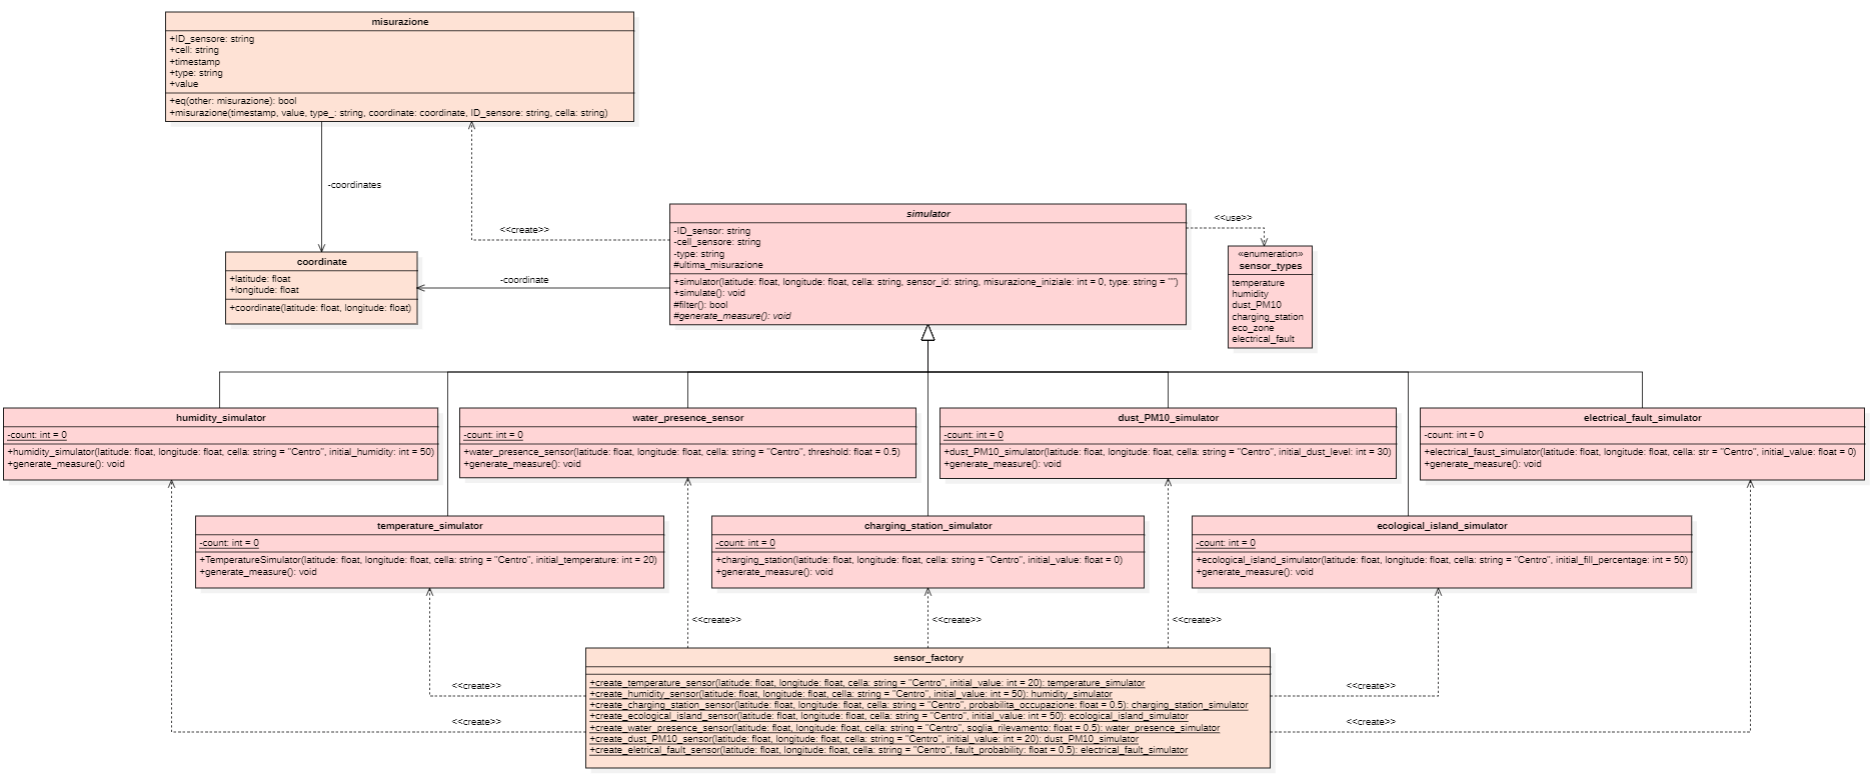
\includegraphics[width=1\textwidth]{../Images/SpecificaTecnica/simulatoriSensori.PNG}
    \caption{Modulo simulatori sensori - innovacity}
    \label{fig: fddf}
\end{figure}

Il processo per il calcolo del punteggio di salute riceve le letture dei sensori attraverso gli agenti di elaborazione dell'applicazione Faust, i quali sono in ascolto sui topic Kafka relativi alle misurazioni di temperatura, umidità e polveri sottili PM10. Ad intervalli regolari, il sistema calcola il punteggio di salute della città basandosi su tali misurazioni. Una volta effettuato il calcolo, il risultato è reso disponibile in un topic Kafka dedicato.
Il modello che racchiude la logica per il calcolo, richiamato a intervalli regolari, è quello attualmente preso in esame.

In sintesi, il modello:
\begin{itemize}
    \item Riceve le misurazioni di temperatura, umidità e polveri sottili dall'agente dell'app Faust.
    \item Riceve da un thread la richiesta ad intervalli regolari di calcolare i punteggi di salute per le celle della città con le misurazioni ottenute in tempo reale.
\end{itemize}

In accordo con l'architettura esagonale, la logica del modello è completamente disaccoppiata dai suoi utilizzatori, i quali interagiscono con il modello tramite specifiche classi adapter. Questo approccio promuove la separazione delle preoccupazioni e favorisce la modularità del sistema. Gli adapter fungono da ponte tra il modello e gli utilizzatori, consentendo una comunicazione fluida e senza dipendenze dirette. Così, eventuali cambiamenti nella logica del modello possono essere implementati senza influenzare gli utilizzatori, garantendo una maggiore flessibilità e manutenibilità del sistema nel suo complesso.

Il presente modulo è concepito per fornire la logica relativa al puro calcolo del punteggio di salute della città. Tale calcolo si basa su un modello che tiene conto delle misurazioni di temperatura, umidità e polveri sottili PM10. Il modello è stato progettato al fine di determinare un punteggio di salute per ciascuna cella della città in cui sono presenti misurazioni delle suddette tipologie.

\paragraph*{Design Pattern Strategy}

Il modello per il calcolo del punteggio di salute è stato ideato mediante l'utilizzo del design pattern Strategy. Tale pattern consente di definire una famiglia di algoritmi, di incapsularli e renderli intercambiabili. Ciò permette di variare l'algoritmo impiegato per il calcolo del punteggio di salute senza incidere sui processi di elaborazione dell'applicazione Faust o sugli altri componenti del sistema. In particolare, l'interfaccia \textit{HealthAlgorithm} stabilisce il contratto che deve essere rispettato da tutti gli algoritmi per il calcolo del punteggio di salute.


Inoltre, un'implementazione del pattern \textit{Strategy} è presente anche negli "Incrementatori". Questi, a partire dalle misurazioni fornite, restituiscono un incremento al punteggio di salute della città. Tale incremento è determinato in base a delle soglie predefinite di temperatura, umidità e polveri sottili PM10, le quali sono definite di default in \textit{health\_constants} ma possono essere impostate al momento della costruzione. In particolare, l'interfaccia \textit{Incrementer} specifica il contratto che deve essere rispettato da tutti gli incrementatori. Vengono implementati tre incrementatori, uno per il calcolo dell'incremento di temperatura, uno per l'umidità e uno per le polveri sottili PM10, come strategie del pattern.

\paragraph{Classi: metodi e attributi}
\begin{itemize}
    \item{\textbf{Interfaccia: \textit{HealthAlgorithm}}}
    \begin{itemize}
    \item \textbf{Metodi: }
    \begin{itemize}
        \item \textbf{generate\_new\_health\_score(): List[MisurazioneSalute] [abstractmethod]} - Un metodo astratto che deve essere implementato nelle sottoclassi. Questo metodo dovrebbe generare un nuovo punteggio di salute.
    \end{itemize}
    \item\textbf{Note}:
        \begin{itemize}
            \item L'interfaccia definisce il contratto per un algoritmo di salute. Le sottoclassi devono implementare il metodo \textit{generate\_new\_health\_score};
            \item Rappresenta la componente "Strategy" del pattern omonimo.
            \item Per rispettare il Single responsibility principle, noto anche come principio di coesione, è stata divisa dalla logica di buffering delle misurazioni presente nella classe astratta \textit{HealthProcessorBuffer} poiché l'utilizzatore \textit{HealthCalculatorThread} non utilizza i metodi per il buffering.
        \end{itemize}
    \end{itemize}
    \item\textbf{Classe astratta: \textit{HealthProcessorBuffer}}
    \begin{itemize}
    \item\textbf{Attributi}:
        \begin{itemize}
        \item \textbf{listaMisurazioni:ListaMisurazioni [private]} - Una lista di oggetti Misurazione.
        \item \textbf{lock:threading.Lock [private]} - Un oggetto lock per gestire l'accesso concorrente alla lista di misurazioni.
    \end{itemize}
    \item \textbf{Metodi: }
    \begin{itemize}
        \item \textbf{add\_misurazione(timestamp, value, type\_, latitude, longitude, ID\_sensore, cella): None [public]} - Aggiunge una nuova misurazione alla lista di misurazioni.
        \item \textbf{clear\_list(): None [public]} - Svuota la lista di misurazioni.
    \end{itemize}
    \item\textbf{Note}:
        \begin{itemize}
               \item La classe astratta definisce un buffer di misurazioni per effettuare il processing su un set di misurazioni. Tale buffer contiene una lista di misurazioni e fornisce metodi per aggiungere misurazioni, ottenere la lista di misurazioni e svuotare la lista.
                \item La logica di buffering e quella dell'algoritmo per il calcolo del punteggio di salute vengono separate in due astrazioni per rispettare il principio di Single Responsibility. Gli utilizzatori di questa classe, i \textit{Processor}, sono interessati esclusivamente al metodo per l'invio del dato al buffer.
                \item La classe astratta definisce un'interfaccia per la comunicazione con gli utilizzatori esterni al modello.
        \end{itemize}
    \end{itemize}
    \item{\textbf{Classe: \textit{HealthCalculator}}}
    \begin{itemize}
    \item\textbf{Attributi}:
        \begin{itemize}
        \item \textbf{tmpInc:TemperatureIncrementer [private]} - Utilizzato per il calcolo dell'incremento di temperatura;
        \item \textbf{umdInc:HumidityIncrementer [private]}; - Utilizzato per il calcolo dell'incremento di umidità;
        \item \textbf{dstPm10Inc:DustPM10Incrementer [private]} - Utilizzato per il calcolo dell'incremento di PM10;
        \item \textbf{temperature\_measure\_type\_naming:string [private]} - Nomenclatura dei tipi di misurazione di temperatura.
        \item \textbf{humidity\_measure\_type\_naming:string [private]} - Nomenclatura dei tipi di misurazione di umidità.
        \item \textbf{ dtsPm10\_measure\_type\_naming:string [private]} - Nomenclatura dei tipi di misurazione di PM10.
        \item \textbf{ healthScore\_measure\_type\_naming:string [private]} - Nomenclatura dei tipi di misurazione di punteggio di salute.
        \item \textbf{lock [private]} - Un oggetto lock per gestire l'accesso concorrente.
    \end{itemize}
    \item \textbf{Metodi: }
    \begin{itemize}
        \item \textbf{generate\_new\_health\_score(): List[MisurazioneSalute] [public]} - Genera e restituisce una nuova lista di punteggi di salute, uno per ogni cella della città di cui sono state fornite misurazioni.
        \item \textbf{calcola\_incremento\_tmp(cella: str, listaMisurazioni): int [private]} - Calcola e restituisce l'incremento della temperatura.
        \item \textbf{calcola\_incremento\_umd(cella: str, listaMisurazioni): int [private]} - Calcola e restituisce l'incremento dell'umidità.
        \item \textbf{calcola\_incremento\_dstPm10(cella: str, listaMisurazioni): int [private]} - Calcola e restituisce l'incremento della polvere PM10.
    \end{itemize}
    \item\textbf{Note}:
        \begin{itemize}
            \item La classe implementa l'interfaccia \textit{HealthAlgorithm} e la classe astratta \textit{HealthProcessorBuffer} per calcolare il punteggio di salute tramite la strategia concreta definita in \textit{generate\_new\_health\_score()} che genera una nuova lista di punteggi di salute.
            \item Questa classe rappresenta il vero cervello del calcolo del punteggio di salute in quanto utilizzatore di tutti gli incrementatori e delle misurazioni bufferizzate per creare una strategia di calcolo.
        \end{itemize}
    \end{itemize}
    \item\textbf{Classe: \textit{Misurazione}}
    \begin{itemize}
        \item   \textbf{Attributi}: 
    \begin{itemize}
        \item \textbf{timestamp:datetime [private]} - Timestamp della misurazione.
        \item \textbf{value:T [private]} - Valore della misurazione.
        \item \textbf{type:str [private]} - Tipo della misurazione.
        \item \textbf{coordinates:Coordinate [private]} - Coordinate della misurazione.
        \item \textbf{ID\_sensore:str [private]} - ID del sensore che ha effettuato la misurazione.
        \item \textbf{cella:str [private]} - Cella in cui è stata effettuata la misurazione.
    \end{itemize}
    \item   \textbf{Metodi}: 
    \begin{itemize}
        \item \textbf{\_\_eq\_\_(other:Misurazione):bool [public]} - Ridefinizione dell'operatore di uguaglianza per confrontare due oggetti Misurazione.
    \end{itemize}
\end{itemize}
    \item\textbf{Classe: \textit{Coordinate}}
    \begin{itemize}
        \item    \textbf{Attributi}: 
    \begin{itemize}
        \item \textbf{latitude:float [private]} - Latitudine della coordinata.
        \item \textbf{longitude:float [private]} - Longitudine della coordinata.
    \end{itemize}
    \item     \textbf{Metodi}: 
    \begin{itemize}
        \item \textbf{\_\_eq\_\_(other:Coordinate):bool [public]} - Ridefinizione dell'operatore di uguaglianza per confrontare due oggetti Coordinate.
    \end{itemize}
\end{itemize}
\item\textbf{Classe: \textit{MisurazioneSalute}}
    \begin{itemize}
    \item\textbf{Attributi}:
        \begin{itemize}
        \item \textbf{timestamp:datetime [private]} - Il timestamp della misurazione di salute.
        \item \textbf{value:float [private]} - Il valore della misurazione di salute.
        \item \textbf{type:string [private]} - Il tipo della misurazione.
        \item \textbf{cella:string [private]} - La cella della misurazione di salute.
    \end{itemize}
    \item\textbf{Note}:
        \begin{itemize}
            \item La classe rappresenta una misurazione di salute. Contiene informazioni sul timestamp, il valore (ovvero il punteggio di salute calcolato), il tipo della misurazione e la cella relativa alla misurazione.
        \end{itemize}
    \end{itemize}
    \item\textbf{Classe: \textit{ListaMisurazioni}}
    \begin{itemize}
    \item\textbf{Attributi}:
        \begin{itemize}
        \item \textbf{list:List[Misurazione] [private]} - Una lista di oggetti Misurazione.
    \end{itemize}
    \item \textbf{Metodi: }
    \begin{itemize}
        \item \textbf{add\_misurazione(timestamp, value, type\_, latitude, longitude, ID\_sensore, cella): None [public]} - Aggiunge una nuova misurazione alla lista.
        \item \textbf{clear\_list(): None [public]} - Svuota la lista di misurazioni.
        \item \textbf{get\_list\_by\_cella\_and\_type(cella: str, tipo\_dato: str): List[Misurazione] [public]} - Restituisce una lista di misurazioni che corrispondono alla cella e al tipo di misurazione specificati (temperatura,umidità,ecc.).
        \item \textbf{get\_unique\_celle(): List[str] [public]} - Restituisce la lista di celle presenti nelle misurazioni senza ripetzioni.
    \end{itemize}
    \item\textbf{Note}:
        \begin{itemize}
            \item La classe rappresenta una lista di misurazioni. Fornisce metodi per aggiungere misurazioni, svuotare la lista, ottenere misurazioni per cella e tipo di misurazioni, e ottenere le celle di cui si hanno misurazioni.
        \end{itemize}
    \end{itemize}
    \item\textbf{Enumerazione: \textit{SensorTypes}}
        \begin{itemize}
            \item \textbf{Costanti}: 
            \begin{itemize}
                \item \textbf{TEMPERATURE:str [public]} - Rappresenta la nomenclatura dei sensore di temperatura.
                \item \textbf{HUMIDITY:str [public]} - Rappresenta la nomenclatura dei sensore di umidità.
                \item \textbf{DUST\_PM10:str [public]} - Rappresenta la nomenclatura dei sensore di "polvere PM10".
                \item \textbf{CHARGING\_STATION:str [public]} - Rappresenta la nomenclatura dei sensore di stato delle colonnine di ricarica.
                \item \textbf{ECOLOGICAL\_ISLAND:str [public]} - Rappresenta la nomenclatura dei sensore di stato riempimento isole ecologica.
                \item \textbf{WATER\_PRESENCE:str [public]} - Rappresenta la nomenclatura dei sensore di presenza d'acqua.
                \item \textbf{ELECTRICAL\_FAULT:str [public]} - Rappresenta la nomenclatura dei sensore di guasti elettrici.
            \end{itemize}

            \item \textbf{Note}:
            \begin{itemize}
                \item L'enumerazione viene utilizzata per centralizzare la gestione della nomenclatura dei tipi di sensori che verrà salvata nelle misurazioni.
            \end{itemize}
        \end{itemize}
\item \textbf{Interfaccia: \textit{Incrementer}}
    \begin{itemize}
    \item \textbf{Metodi: }
    \begin{itemize}
        \item \textbf{get\_incrementation(misurazioni: List[Misurazione]): int [abstractmethod]} - Un metodo astratto che deve essere implementato nelle sottoclassi. Questo metodo calcola e restituire un incremento basato sulla lista di misurazioni fornita.
    \end{itemize}
    \item\textbf{Note}:
        \begin{itemize}
            \item L'interfaccia definisce il contratto per un incrementatore. Le sottoclassi devono implementare il metodo \textit{get\_incrementation()}.
            \item Rappresenta la componente "Strategy" del pattern omonimo.
        \end{itemize}
    \end{itemize}
    \item \textbf{Classe: \textit{TemperatureIncrementer}}
    \begin{itemize}
    \item \textbf{Attributi}:
        \begin{itemize}
        \item \textbf{upper\_health\_soglia:int [private]} - La soglia superiore di benessere per la temperatura;
        \item \textbf{under\_health\_soglia:int [private]} - La soglia inferiore di benessere per la temperatura.
    \end{itemize}
    \item \textbf{Metodi: }
    \begin{itemize}
        \item \textbf{get\_incrementation(misurazioni: List[Misurazione]): int [public]} - Calcola e restituisce un incremento basato sulle sole misurazioni di temperatura della lista fornita.
    \end{itemize}
    \item\textbf{Note}:
        \begin{itemize}
            \item La classe implementa l'interfaccia \textit{Incrementer};
            \item I valori di default per le soglie vengono presi dall'enumerazione \textit{HealthConstant} altrimenti sono impostabili alla costruzione.
            \item Rappresenta una strategia concreta del pattern \textit{Strategy} per il calcolo dell'incremento di temperatura.
        \end{itemize}
    \end{itemize}
    \item{\textbf{Classe: \textit{HumidityIncrementer}}}
    \begin{itemize}
    \item\textbf{Attributi}:
        \begin{itemize}
        \item \textbf{upper\_health\_soglia:int [private]} - La soglia superiore di benessere per l'umidità;
        \item \textbf{under\_health\_soglia:int [private]} - La soglia inferiore di benessere per l'umidità.
    \end{itemize}
    \item \textbf{Metodi: }
    \begin{itemize}
        \item \textbf{get\_incrementation(misurazioni: List[Misurazione]): int [public]} - Calcola e restituisce un incremento basato sulle sole misurazioni di umidità della lista fornita.
    \end{itemize}
    \item\textbf{Note}:
        \begin{itemize}
            \item La classe implementa l'interfaccia \textit{Incrementer};
            \item I valori di default per le soglie vengono presi dall'enumerazione \textit{HealthConstant} altrimenti sono impostabili alla costruzione.
            \item Rappresenta una strategia concreta del pattern \textit{Strategy} per il calcolo dell'incremento di umidità.
        \end{itemize}
    \end{itemize}\item{\textbf{Classe: \textit{DustPM10Incrementer}}}
    \begin{itemize}
    \item \textbf{Metodi: } 
    \begin{itemize}
        \item \textbf{get\_incrementation(misurazioni: List[Misurazione]): int [public]} - Calcola e restituisce un incremento basato sulle sole misurazioni di polveri sottili della lista fornita.
    \end{itemize}
    \item\textbf{Note}:
        \begin{itemize}
            \item La classe implementa l'interfaccia \textit{Incrementer};
            \item Rappresenta una strategia concreta del pattern \textit{Strategy} per il calcolo dell'incremento di polveri sottili PM10.
            \item A differenza degli altri \textit{Incrementer}, \textit{DustPM10Incrementer} non definisce soglie di benessere in quanto è scontato che il valore ottimale di inquinamento è zero.
        \end{itemize}
    \end{itemize}

\end{itemize}

\subsubsection{Modulo Writer}
Il modulo Writer è lo stesso di quello descritto in \ref*{sec:writersModule} e viene nella sua totalità riutilizzato per la scrittura dei punteggi di salute calcolati.
Non viene riportata la strategia di scrittura su di una lista poichè non ne è stato ritenuto necessario l'utilizzo.

\paragraph*{Classi: metodi e attributi}
Tutte le informazioni sono già state esposte in: \ref*{sec:writersModule}.

\subsubsection{Modulo Threading/Scheduling}
\begin{figure}[H]
    \centering
    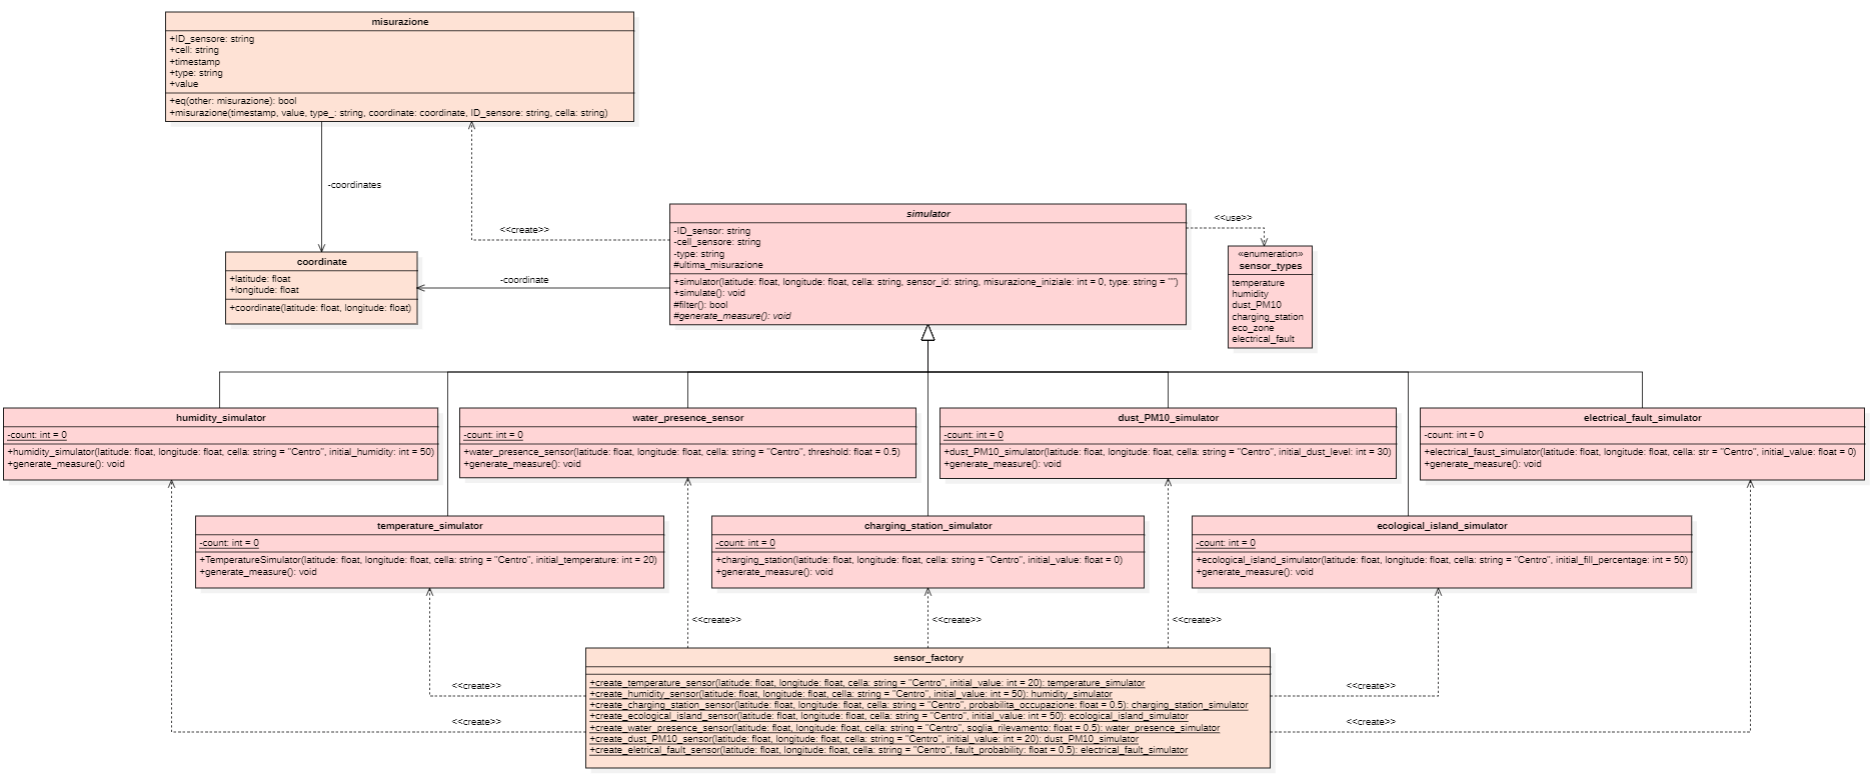
\includegraphics[width=1\textwidth]{../Images/SpecificaTecnica/simulatoriSensori.PNG}
    \caption{Modulo simulatori sensori - innovacity}
    \label{fig: fddf}
\end{figure}

Questo modulo si occupa di integrare la logica di Scheduling e Threading per il calcolo periodico del punteggio di salute della città e quella di scrittura/invio di \textit{Writable}. In particolare, fornisce un'implementazione di un thread che, a intervalli regolari, richiama il calcolo del punteggio di salute della città. Successivamente, utilizzando il modulo "Writer", adatta le misurazioni di salute ottenute all'interfaccia per renderle un oggetto che implementa \textit{Writable}. Pertanto, questo modulo è utilizzatore del modello per il calcolo del punteggio di salute e del modulo di Writer.
In sintesi, il modulo:
    \begin{enumerate}
        \item Richiama l'algoritmo per calcolo del punteggio di salute della città a intervalli regolari;
        \item Scrive il risultato ottenuto sul topic Kafka dedicato.
    \end{enumerate}

\paragraph*{Dependecy Inversion principle}
Il modulo di scheduling e threading dipende dall'astrazione dell'interfaccia del modello per il calcolo del punteggio di salute e del modulo di Writer, invece di dipendere direttamente dalle implementazioni concrete di questi moduli. Ciò consente una maggiore flessibilità e facilità di manutenzione, poiché il modulo di scheduling e threading non è vincolato a implementazioni specifiche, ma può essere facilmente adattato per utilizzare diverse implementazioni che soddisfano lo stesso contratto.

In sostanza, seguendo il principio di Inversione delle Dipendenze, il modulo di scheduling e threading si concentra sull'utilizzo di interfacce o astrazioni, piuttosto che sulle implementazioni concrete, rendendo il sistema più modulare, scalabile e facilmente estendibile.

\paragraph*{Classi: metodi e attributi}
\begin{itemize}
    \item{\textbf{Classe: \textit{HealthCalculatorThread}}}
    \begin{itemize}
    \item\textbf{Attributi}:
        \begin{itemize}
        \item \textbf{healthCalculator: HealthAlgorithm [private]} - Un implementatazione dell'interfaccia \textit{HealthAlgorithm}, ovvero una strategia per il calcolo del punteggio.
        \item \textbf{frequency: float [private]} - La frequenza con cui il thread genera nuovi punteggi di salute.
        \item \textbf{is\_running: bool [private]} - Un flag che indica se il thread è in esecuzione.
        \item \textbf{data\_to\_generate: int [private]} - Il numero di misurazioni di salute da generare.
        \item \textbf{writers: Writer [private]} - Un oggetto della classe Writer. (Singolo scrittore o albero, Composite pattern)
    \end{itemize}
    \item \textbf{Metodi: }
    \begin{itemize}
        \item \textbf{run(): None [public]} - Esegue il thread, generando nuovi punteggi di salute a una certa frequenza.
        \item \textbf{stop(): None [public]} - Ferma l'esecuzione del thread.
    \end{itemize}
    \item\textbf{Note}:
        \begin{itemize}
            \item La classe estende la classe \textit{threading.Thread}.
            \item Se \textit{data\_to\_generate} è < 0 genera misurazioni di salute finchè il thread non viene interroto dall'esterno.
            \item   Grazie al pattern \textit{Strategy} è possibile cambiare agevolmente l'algoritmo volto al calcolo del punteggio di salute della città.
        \end{itemize}
    \end{itemize}
\end{itemize}

\subsubsection{Modulo Processing}
Per garantire un'interfaccia uniforme per i metodi di elaborazione dei dati provenienti da Kafka tramite Faust e per stabilire un canale di comunicazione con il modello per il calcolo del punteggio di salute, viene sviluppato il modulo di Processing. Questo modulo offre l'interfaccia target denominata \textit{Processor}, e un adapter a \textit{Processor} per l'invio delle misurazioni al modello per il calcolo del punteggio di salute, denominato \textit{HealthModelProcessorAdapter}.

\paragraph*{Design Pattern Object Adapter}
Nel contesto dell'applicazione Faust, all'interno del ruolo svolto dagli agenti, ogni volta che una misurazione viene ricevuta, viene invocato il metodo \textit{process\_measure()} dell'implementazione dell'interfaccia \textit{Processor}, denominata \textit{HealthModelProcessorAdapter}. In particolare, \textit{HealthModelProcessorAdapter} adatta la classe astratta \textit{HealthModelBuffer}, che rappresenta un buffer di misurazioni utilizzato per eseguire il calcolo periodico del punteggio di salute della città, all'interfaccia \textit{Processor}.

Questo pattern consente di incapsulare le logiche di elaborazione e di rendere il modello indipendente dall'implementazione specifica dell'applicazione Faust. Allo stesso tempo, facilita la sostituzione dell'operazione di elaborazione eseguita su ogni misurazione dagli agenti grazie al contratto dell'interfaccia \textit{Processor}.
\paragraph*{Classi: metodi e attributi}
\begin{itemize}
    \item{\textbf{Interfaccia: \textit{Processor}}}
    \begin{itemize}
    \item\textbf{Metodi: }
    \begin{itemize}
        \item \textbf{process(misurazione: FaustMeasurement): None [public, abstract]} - Un metodo astratto che deve essere implementato nelle sottoclassi. Questo metodo elabora una misurazione.
    \end{itemize}
    \item\textbf{Note}:
        \begin{itemize}
            \item  Le sottoclassi devono implementare il metodo astratto \textit{process()} definendo la propria operazione da effettuare su ogni misurazione ricevuta dai topic di iscrizione.
            \item Rappresenta la componente "Target" del pattern \textit{Object Adapter}.
            \item L'interfaccia è stata progettata per garantire un'interfaccia uniforme per i metodi di elaborazione dei dati provenienti da Kafka tramite Faust.
            \item Rappresenta un contratto per l'elaborazione di misurazioni.
            \item Gli agenti in ascolto sul topic utilizzeranno un implementatazione di \textit{Processor} per effettuare l'elaborazione delle misurazioni ottenute.
        \end{itemize}
    \end{itemize}
    \item{\textbf{Classe: \textit{FaustMeasurement}}}
    \begin{itemize}
    \item\textbf{Attributi}:
        \begin{itemize}
        \item \textbf{timestamp: str} - Il timestamp della misurazione.
        \item \textbf{value: float} - Il valore della misurazione.
        \item \textbf{type: str} - Il tipo della misurazione.
        \item \textbf{latitude: float} - La latitudine della misurazione.
        \item \textbf{longitude: float} - La longitudine della misurazione.
        \item \textbf{ID\_sensore: str} - L'ID del sensore che ha effettuato la misurazione.
        \item \textbf{cella: str} - La cella della misurazione.
    \end{itemize}
    \item\textbf{Note}:
        \begin{itemize}
            \item La classe \textit{FaustMeasurement} definita utilizzando \textit{faust.Record} rappresenta un singolo record di misurazione proveniente da un sensore in un'applicazione Faust basata su Python
            \item Faust si occupa automaticamente della conversione dei dati in formato JSON in base agli attributi definiti, facilitando la trasmissione e la ricezione dei dati nei topic Kafka.
            \item È possibile definire la validazione dei dati in ingresso per garantire l'integrità e la coerenza delle misurazioni.
            \item \textbf{In sintesi}:
            Questa classe viene utilizzata in un'applicazione Faust per definire il tipo di dati atteso nei topic Kafka. I dati provenienti dai sensori, contenenti timestamp, valore, tipo, coordinate geografiche, identificativo del sensore e eventuale cella di appartenenza, verranno convertiti in oggetti di tipo FaustMeasurement prima di essere elaborati dall'applicazione.
        \end{itemize}
    \end{itemize}
    \item{\textbf{Classe: \textit{HealthModelProcessorAdapter}}}
    \begin{itemize}
    \item\textbf{Attributi}:
        \begin{itemize}
        \item \textbf{healthCalculator: HealthProcessorBuffer} - Un implementazione di HealthProcessorBuffer.
    \end{itemize}
    \item \textbf{Metodi: }
    \begin{itemize}
        \item \textbf{process(misurazione: FaustMeasurement): None [public, async]} - Aggiunge la misurazione all'oggetto \textit{HealthProcessorBuffer} adattando \textit{FaustMeasurement} alla porta di accesso fornita da \textit{HealthProcessorBuffer} per l'elaborazione volta al calcolo del punteggio di salute.
    \end{itemize}
    \item\textbf{Note}:
        \begin{itemize}
            \item La classe implementa l'interfaccia \textit{Processor}. Implementa il metodo astratto \textit{process()} per aggiungere/adattare la misurazione del tipo \textit{FaustMeasurement} ad un implementatazione di \textit{HealthProcessorBuffer}.
            \item Rappresenta la componente "Adapter" del pattern \textit{Object Adapter}.
        \end{itemize}
    \end{itemize}
\end{itemize}


\subsection{Configurazione Database}
Si è optato per l'utilizzo di ClickHouse per il salvataggio dei dati, le motivazioni sono descritte nella sezione \ref{sec:clickHouse}. In particolare, per ogni sensore dei quali si desidera memorizzare i dati, viene creata una tabella che acquisisce i dati dal relativo topic Kafka.
Le tipologie di sensori cui misurazioni si vogliono trattare nel progetto sono:
\begin{itemize}
    \item Sensori di temperatura;
    \item Sensori di umidità;
    \item Sensori di rilevamento polveri sottili; 
    \item Sensori stato riempimento isole ecologiche;
    \item Sensori di stato occupazione colonnine di ricarica;
    \item Sensori di guasti elettrici;
    \item Sensori del livello dell'acqua.
\end{itemize}

La configurazione del database ClickHouse è stata cruciale nella progettazione, poiché un'adeguata ottimizzazione consente di garantire prestazioni ottimali per un sistema orientato al tempo reale e in grado di gestire analisi su enormi volumi di dati.


\subsubsection{Funzionalità Clickhouse utilizzate}
\paragraph{Materialized Views}
Le Materialized Views in ClickHouse sono un meccanismo potente per migliorare le prestazioni delle query e semplificare l'accesso ai dati. Funzionano mantenendo una copia fisica dei risultati di una query di selezione, che viene quindi memorizzata su disco. Questa copia è aggiornata periodicamente in base ai dati sottostanti.

\paragraph*{Utilizzi Principali delle Materialized Views}
\begin{itemize}
    \item \textbf{Calcolo aggregazioni e popolamento tabelle}:Spesso le delle materialized Views sono state utilizzate per calcolare aggregazioni su dati e quindi popolare altre tabelle con i risultati aggregati. Ad esempio, nel caso specifico in cui una Materialized View calcola la media delle temperature per ogni sensore ogni secondo, i risultati di questa vista possono essere utilizzati per popolare una tabella principale contenente i dati di temperatura aggregati, aggiornando i valori di temperatura medi per ogni sensore ogni secondo;
    \item \textbf{Ottimizzazione delle Prestazioni}: memorizzando i risultati di una query complessa, le Materialized Views consentono di eseguire rapidamente le Query successive senza dover ricalcolare i dati ogni volta. Ciò è particolarmente utile in applicazioni che richiedono interrogazioni frequenti su grandi volumi di dati;
    \item \textbf{Decomposizione delle \textit{Query} Complesse}: le Materialized Views consentono di decomporre query complesse in passaggi più semplici e riutilizzabili, migliorando la leggibilità del codice e semplificando lo sviluppo e la manutenzione delle query.
\end{itemize}



\paragraph{MergeTree}\label{sec:MergeTree}
Link alla documentazione: \href{https://clickhouse.com/docs/en/engines/table-engines/mergetree-family/mergetree#mergetree}{ClickHouse - MergeTree}.\newline
MergeTree è uno dei motori di tabella più potenti e utilizzati in ClickHouse, noto per la sua capacità di gestire e memorizzare grandi volumi di dati in modo efficiente. È una scelta ideale per applicazioni che richiedono l'archiviazione e l'analisi di dati cronologicamente ordinati, come i dati di log o di monitoraggio. L'architettura di MergeTree organizza i dati in parti, ciascuna contenente una serie di punti dati ordinati cronologicamente. Questa organizzazione ottimizzata consente di eseguire rapidamente le query che richiedono l'accesso a dati specifici all'interno di un intervallo di tempo definito, garantendo prestazioni elevate anche su grandi dataset. Oltre alla gestione efficiente dei dati, MergeTree supporta funzionalità avanzate come la compressione dei dati e la gestione automatica delle partizioni. Queste caratteristiche consentono di ottimizzare ulteriormente le prestazioni e la gestione complessiva dei dati, rendendo MergeTree una scelta affidabile per una vasta gamma di scenari di utilizzo in ClickHouse.



\paragraph{Time To Live in ClickHouse} \label{sec:RollupTTL}
Link alla documentazione: \href{https://clickhouse.com/docs/en/guides/developer/ttl#implementing-a-rollup}{ClickHouse - Implementing a Rollup}\newline
In ClickHouse, la funzionalità TTL (Time To Live) è un elemento chiave per gestire grandi volumi di dati in modo efficiente e garantire la pulizia automatica di informazioni obsolete o non più rilevanti. \\
Quando si specifica il motore Rollup per definire una tabella in ClickHouse, si abilita la creazione di tabelle che supportano il TTL. Questo consente di impostare un periodo temporale dopo il quale i dati saranno eliminati automaticamente dalla tabella. La struttura a Rollup organizza i dati in parti, ciascuna contenente una serie di punti dati ordinati cronologicamente. Il TTL può essere configurato per ciascuna parte dei dati, offrendo un controllo preciso sulla conservazione delle informazioni nel tempo. Questa flessibilità è particolarmente utile per applicazioni che richiedono la conservazione di dati storici per un periodo limitato, come ad esempio i dati di log o di monitoraggio. \newline
Un esempio di come potrebbe può venire utilizzato il motore Rollup per il TTL in ClickHouse è il seguente:
\begin{verbatim}
    TTL toDateTime(timestamp) + INTERVAL 1 MONTH
\end{verbatim}
L'uso del TTL di tipo Rollup in questo contesto è cruciale per garantire che la tabella rimanga efficiente e gestibile nel tempo, eliminando automaticamente i dati più vecchi e non più necessari dopo un periodo di tempo specificato. Questo aiuta a ottimizzare le prestazioni complessive del sistema e a gestire in modo efficiente i grandi volumi di dati accumulati nel tempo.


\paragraph{Partition}\label{sec:Partition}
Link alla documentazione: \href{https://clickhouse.com/docs/en/engines/table-engines/mergetree-family/mergetree#partition-by}{ClickHouse - Partitioning}.\\
Le partizioni sono una funzionalità fondamentale di ClickHouse che consente di organizzare in modo efficiente e gestire grandi volumi di dati. Questa caratteristica permette di suddividere i dati in gruppi logici in base a criteri specifici, come il valore di una colonna o un intervallo di tempo. Grazie a questa organizzazione ottimizzata, le query che richiedono l'accesso a dati specifici all'interno di una partizione possono essere eseguite rapidamente, garantendo prestazioni elevate anche su dataset di grandi dimensioni.\\
L'utilizzo delle partizioni nel nostro contesto viene giustificato dall'utilizzo di un TTL (Time To Live), infatti l'utilizzo combinato di queste due funzionalità consente:
\begin{itemize}
    \item Una gestione efficace dei dati nel tempo;
    \item Migliori prestazioni del sistema;
    \item Una semplificazione nella manutenzione del database.
\end{itemize}
Il partizionamento basato sul timestamp è una pratica comune in ClickHouse, poiché consente di organizzare i dati in partizioni in base al periodo temporale, ad esempio mensilmente. Questo approccio ottimizza l'archiviazione e facilita l'analisi dei dati di serie temporali, come le temperature o i log di eventi. Grazie a questa struttura, le query che coinvolgono dati all'interno di specifici intervalli temporali diventano più efficienti, consentendo un accesso rapido e una migliore analisi dei dati.




    
\paragraph{Projection}\label{sec:projections}
Link alla documentazione: \href{https://clickhouse.com/docs/en/sql-reference/statements/alter/projection}{https://clickhouse.com/docs/en/sql-reference/statements/alter/projection}\newline
Le proiezioni memorizzano i dati in un formato che ottimizza l'esecuzione delle \textit{Query}, questa caratteristica è utile per:

\begin{itemize}
    \item Eseguire \textit{Query} su una colonna che non fa parte della chiave primaria;
    \item Pre-aggregare colonne, riducendo sia i calcoli che l'I/O.
\end{itemize}

Puoi definire una o più proiezioni per una tabella e durante l'analisi della \textit{Query} la proiezione con meno dati da esaminare sarà selezionata da ClickHouse senza modificare la \textit{Query} fornita dall'utente.

\paragraph*{Utilizzo dello spazio su disco}
\textbf{Attenzione:} le proiezioni creeranno internamente una nuova tabella nascosta, ciò significa che saranno necessari più I/O e spazio su disco. Ad esempio, se la proiezione ha definito una chiave primaria diversa, tutti i dati dalla tabella originale verranno duplicati.

\subsubsection{Integrazione tramite Kafka Engine in ClickHouse}
ClickHouse supporta l'integrazione con Kafka tramite Kafka Engine, permettendo la lettura dei dati da un topic Kafka e il loro salvataggio in una tabella ClickHouse. Tale funzionalità riveste un'importanza notevole per applicazioni che richiedono l'elaborazione in tempo reale di dati provenienti da fonti esterne, una necessità frequente nel contesto del monitoraggio urbano. L'integrazione con Kafka consente l'acquisizione e la memorizzazione efficiente dei dati, garantendo prestazioni elevate anche su grandi volumi di dati.\\
Kafka Engine è progettato per il recupero di dati una sola volta. Ciò significa che una volta che i dati vengono interrogati da una tabella Kafka, vengono considerati consumati dalla coda. Pertanto, non si dovrebbero mai selezionare dati direttamente da una tabella di Kafka Engine, ma utilizzare invece una vista materializzata. Una vista materializzata viene attivata una volta che i dati sono disponibili in una tabella di Kafka Engine. Automaticamente sposta i dati da una tabella Kafka a una tabella di tipo MergeTree o Distributed. Quindi, sono necessarie almeno 3 tabelle:
\begin{itemize}
  \item La tabella di origine del motore Kafka;
  \item La tabella di destinazione (famiglia MergeTree o distribuita);
  \item Vista materializzata per spostare i dati;
\end{itemize}
\begin{figure}[H]
  \centering
  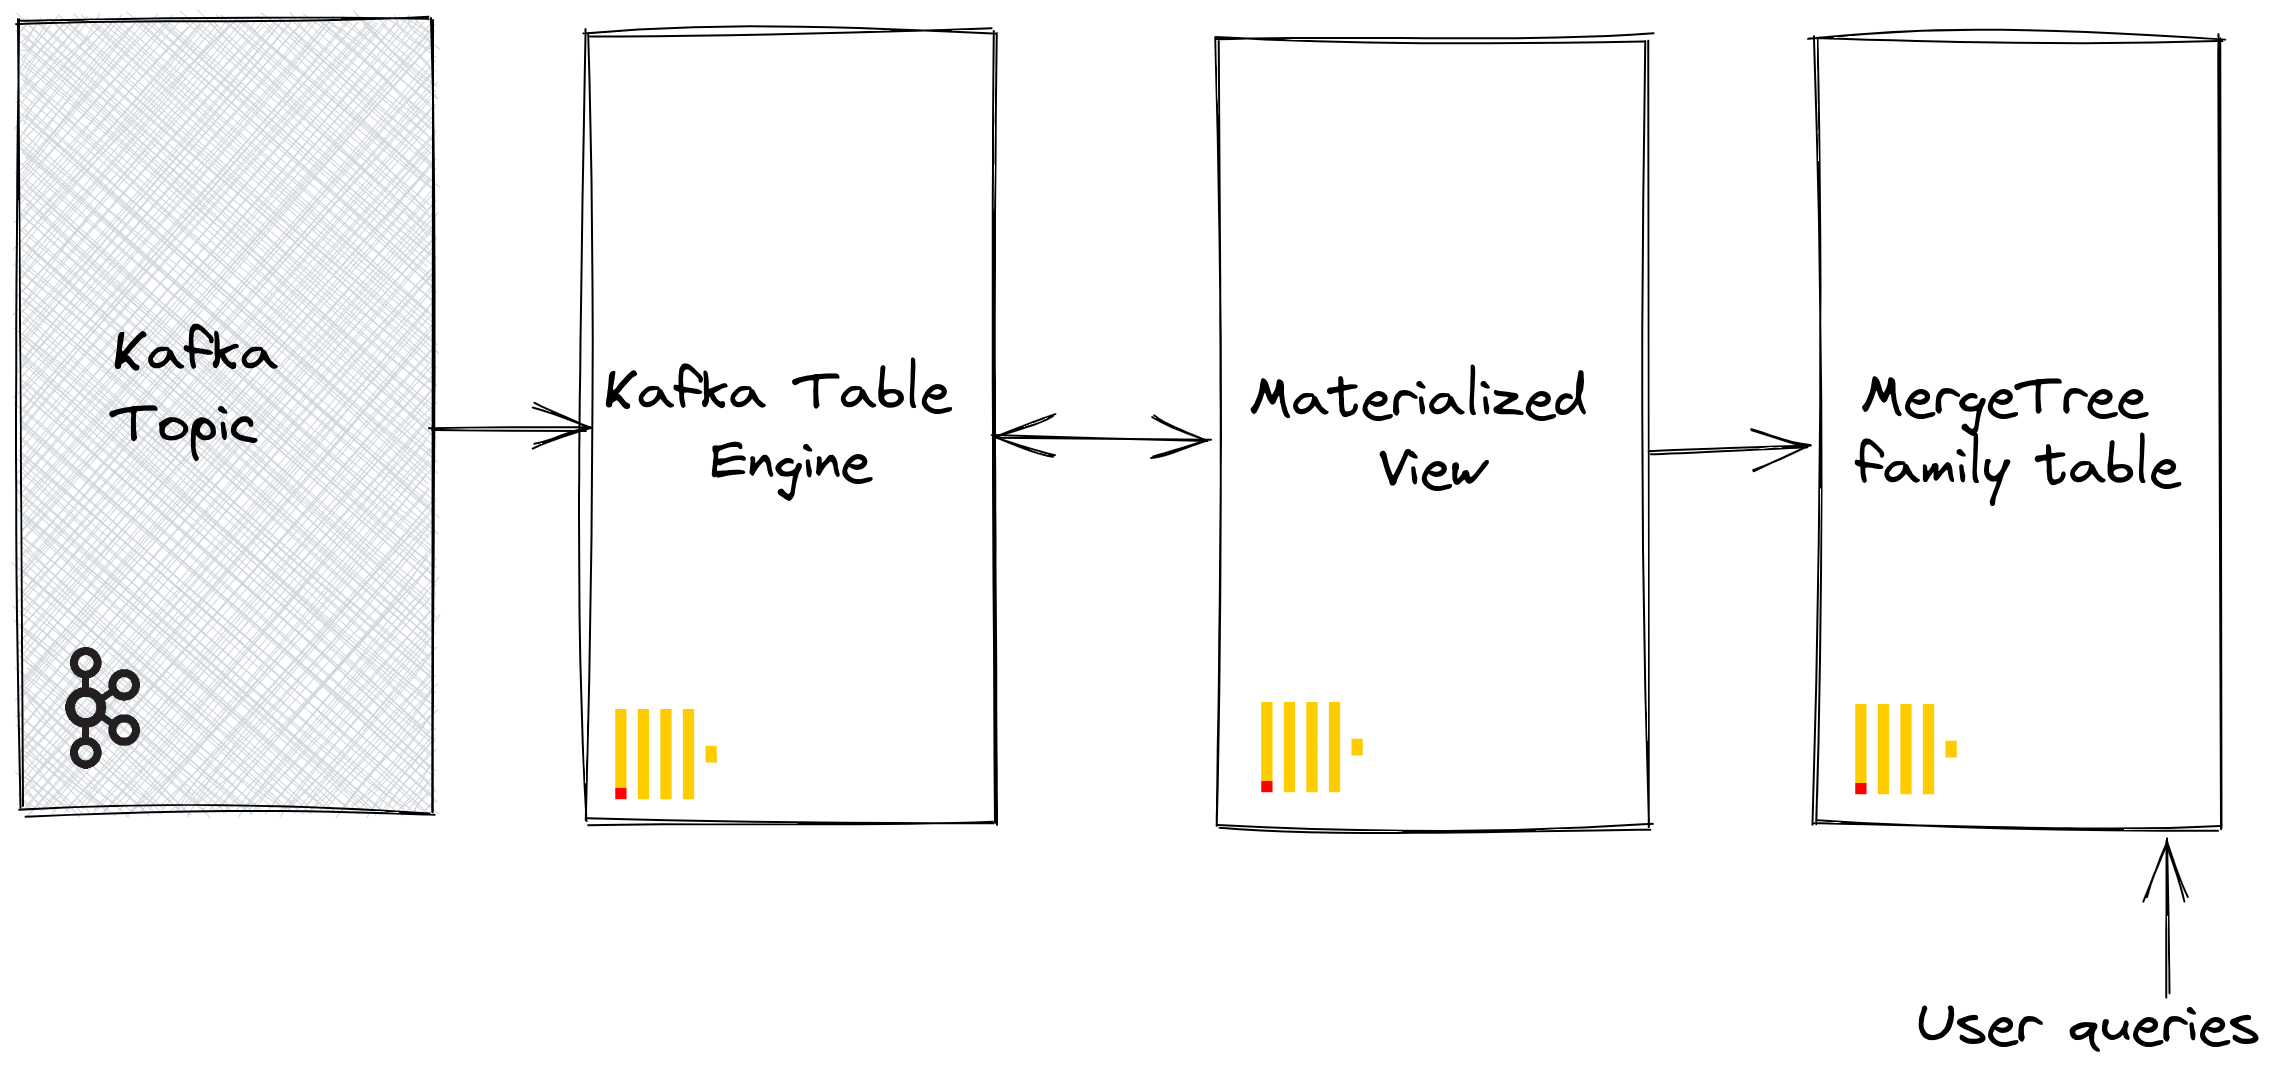
\includegraphics[width=.7\textwidth]{../Images/SpecificaTecnica/kafka_engine_architecture.png}
  \caption{Architettura di Kafka Engine in ClickHouse}
  \label{fig:sensorKafka}
\end{figure}

\subsubsection{Trasferimento dati tramite Materialized View}
Una materialized view funge da ponte tra la fonte dei dati (Kafka Engine) e la destinazione dei dati (MergeTree). Quando nuovi dati vengono scritti nella tabella Kafka Engine, la materialized view viene attivata automaticamente.\\
La materialized view esegue una query sulla tabella Kafka Engine per selezionare i dati più recenti. Una volta selezionati, questi dati vengono inseriti nella tabella di destinazione (ad esempio, una tabella MergeTree). Questo processo avviene in modo automatico e immediato, senza bisogno di intervento manuale.\\
In pratica, la materialized view si assicura che la tabella di destinazione sia sempre aggiornata con i dati più recenti presenti nella tabella Kafka Engine. Questo offre numerosi vantaggi:
\begin{itemize}
  \item \textbf{Automatizzazione del processo}: Non è necessario eseguire manualmente operazioni di trasferimento dati da una tabella all'altra. La materialized view si occupa di tutto in modo automatico;
  \item \textbf{Efficienza}: Il trasferimento dei dati avviene in tempo reale, garantendo che la tabella di destinazione sia sempre allineata con la fonte dei dati senza ritardi;
  \item \textbf{Ottimizzazione delle risorse}: Il processo di trasferimento dei dati è gestito in modo efficiente, utilizzando al meglio le risorse disponibili e garantendo prestazioni elevate.
\end{itemize}
Nel contesto specifico, le materialized view sono responsabili di eseguire controlli sui dati, come ad esempio la verifica della loro correttezza ed affidabilità nel contesto di utilizzo, prima di inserirli nella tabella di destinazione. Questo processo assicura che i dati siano sempre affidabili e pronti per l'analisi, senza la necessità di ulteriori operazioni di pulizia o preparazione.\\
Per esempio, nel caso dei dati di umidità raccolti da sensori in un'area urbana, la materialized view potrebbe eseguire controlli per assicurarsi che i valori rientrino all'interno di un intervallo plausibile e che non ci siano discrepanze improbabili. Ciò garantirebbe che i dati di umidità inseriti nella tabella di destinazione siano accurati e affidabili per l'analisi meteorologica o ambientale.


\subsubsection{Tabella di origine di Kafka Engine per un sensore generico}
Le tabelle del database impiegate per registrare le misurazioni di ciascuna tipologia di sensore presentano una configurazione sostanzialmente simile, differenziandosi principalmente per il tipo di dato della colonna relativa alla misurazione e per il \textit{topic} di riferimento utilizzato per ottenere le misurazioni.
Nello specifico per ogni sensore si avrà la seguente tabella Clickhouse:
\begin{figure}[H]
    \centering
    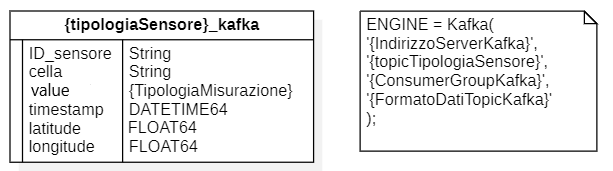
\includegraphics[width=.6\textwidth]{../Images/SpecificaTecnica/sensorType_kafka.PNG}
    \caption{Tabella sensore generico per il reperimento da kafka - ClickHouse}
    \label{fig:sensorKafka}
  \end{figure}

    La tabella è configurata con il motore di storage \textit{Kafka}, il che significa che i dati verranno letti da un \textit{topic Kafka}. 

    I campi sono:
    \begin{itemize}
        \item \textbf{ID\_sensore}: un campo di tipo \textit{String} che identifica univocamente il sensore che ha effettuato la misurazione;
        \item \textbf{cella}: un campo di tipo \textit{String} che rappresenta la cella della città in cui è stata effettuata la misurazione;
        \item \textbf{value}: un campo di tipo variabile a seconda del tipo di misurazione che contiene il valore della temperatura;
        \item \textbf{timestamp}: campo di tipo \textit{DATETIME64} che rappresenta il timestamp della misurazione della temperatura;
        \item \textbf{latitude}: un campo di tipo \textit{Float64} che rappresenta la latitudine del luogo dove è stata effettuata la misurazione;
        \item \textbf{longitude}: un campo di tipo \textit{Float64} che rappresenta la longitudine del luogo dove è stata effettuata la misurazione.
    \end{itemize}

    Mentre i parametri esposti racchiusi da parentesi graffe variano per ogni tipolgia di sensore correlato alla misurazione e sono:
    \begin{itemize}
        \item \textbf{tipologiaSensore}: viene sostituito con la tipologia del sensore che effettua le misurazioni salvate nella tabella; (ex. temperatures)
        \item \textbf{TipoDatoMisurazione}: viene sostituito con il tipo del dato che rappresenta la misurazione (ex. Float32, UInt8);
        \item \textbf{IndirizzoServerKafka}: specifica l'indirizzo del server Kafka.
        Nel nostro caso il server Kafka è in esecuzione su un container \textit{Docker} raggiungibile tramite l'indirizzo:
         \textit{'kafka:9092'};
        \item \textbf{topicTipologiaSensore}: specifica il nome del topic Kafka da cui leggere i dati (ex.temperature);
        \item \textbf{ConsumerGroupKafka}: specifica il nome del consumer group Kafka che verrà utilizzato per leggere i messaggi dal topic \textit{Kafka} denominato 'temperature'.
        Un consumer group in \textit{Kafka} è un gruppo di consumatori che lavorano insieme per consumare i messaggi da uno o più topic. Ogni messaggio inviato a un \textit{topic Kafka} può essere consumato da uno dei consumatori nel gruppo. I consumer all'interno di uno stesso gruppo condividono l'elaborazione dei messaggi all'interno dei topic: ogni messaggio viene elaborato da uno e un solo consumatore all'interno del gruppo. Nel nostro caso sarà sempre '\textit{CG\_Clickhouse\_1}' per indicare il servizio di salvataggio \textit{Clickhouse}.
        \item \textbf{FormatoDatiTopicKafka}: specifica il formato dei dati nel \textit{topic Kafka}. Nel nostro caso, i dati sono nel formato JSONEachRow, che è un formato di serializzazione JSON di \textit{ClickHouse} che consente di scrivere o leggere record JSON separati da una riga. Quindi avremo che <<FormatoDatiTopicKafka>> = JSONEachRow.
        \item \textbf{KafkaSkipBrokenMessages}: specifica il numero di errori da tollerare durante il parsing dei messaggi, configurato a livello di tabella, rappresenta la quantità massima di errori accettabili che il sistema può gestire durante il processo di analisi dei messaggi. Questo parametro consente di regolare il livello di tolleranza agli errori a livello di tabella, offrendo la possibilità di controllare quanto il sistema debba essere flessibile nell'interpretazione dei dati.
    \end{itemize}

    
\subsubsection{Misurazioni temperatura} \label{sec:tab_temperatures}
Di seguito viene fornita la configurazione riguardante il salvataggio delle misurazioni di temperatura:
\paragraph{Tabella: temperatures\_kafka}
\begin{figure}[H]
    \centering
    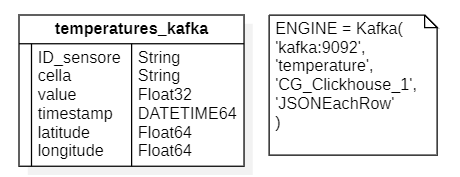
\includegraphics[width=1\textwidth]{../Images/SpecificaTecnica/temperatures_kafka.PNG}
    \caption{Tabella temperatures\_kafka - ClickHouse}
    \label{fig:temperaturesKafka}
  \end{figure}

Il dato della misurazione è di tipo Float32, l'equivalente di float nel linguaggio \textit{C}.
Il topic kafka per ottenere i dati è: \textit{temperature}.

Considerando la possibilità di ricevere molteplici misurazioni dei dati di temperatura all'interno di un singolo secondo di tempo, si procede alla creazione della seguente tabella e alla materialized view correlata, il cui obiettivo è aggregare le misurazioni di temperatura per ridurle ad una singola misurazione per secondo.

\paragraph{Tabella: temperatures}
\begin{figure}[H]
    \centering
    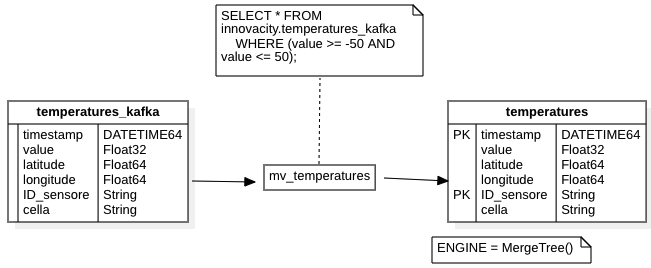
\includegraphics[width=1\textwidth]{../Images/SpecificaTecnica/temperatures.PNG}
    \caption{Tabella temperatures - ClickHouse}
    \label{fig:temperatures}
  \end{figure}

   
    
    \paragraph{Projections per misurazioni di temperatura} \label{sec:temp_projections}
    Durante la fase di progettazione, è stata posta particolare attenzione all'utilizzo delle tabelle appena descritte e alle richieste che verranno formulate su di esse. È emerso, considerando il requisito di suddividere la città in una serie di celle e specificare la cella di origine della misurazione,che la filtrazione delle misurazioni per celle diventerà una richiesta effettuata con frequenza al database.
    Si è giunti quindi all'utilizzo delle \textit{PROJECTIONS}, descritte nella sezione \ref{sec:projections}.
    \vspace{0,3cm}
    \begin{lstlisting}[caption={Esempio di proiezione e materializzazione in una tabella}, captionpos=b]
      --Projection per tabella temperatures
      ALTER TABLE innovacity.temperatures ADD PROJECTION tmp_sensor_cell_projection (SELECT * ORDER BY cella);
      ALTER TABLE innovacity.temperatures MATERIALIZE PROJECTION tmp_sensor_cell_projection;
  \end{lstlisting}
    \vspace{0,3cm}
    La proiezione ci permetterà di filtrare per \textit{cella} e \textit{timestamp} rapidamente, anche se nella tabella originale queste non sOno definite come \textit{PRIMARY\_KEY}.


    \paragraph{Analisi benefici delle Projections}\label{sec:temp_projections_benefici}
    L'aggiunta delle \textit{PROJECTIONS} ha portato risultati di estremo rilievo di seguito esposti.
    Prendendo una \textit{Query} tipo svolta per l'analisi da \textit{Grafana}:
    
    \begin{lstlisting}[caption={Query tipica - Grafana}, captionpos=b]
      SELECT ID_sensore, avgMerge(value) AS value, timestamp
      FROM innovacity.temperatures
      WHERE (cella IN ('Arcella')) AND ((timestamp >= toDateTime64(1708338633507 / 1000, 3)) AND (timestamp <= toDateTime64(1708338933507 / 1000, 3) + INTERVAL 1 DAY))
      GROUP BY timestamp, ID_sensore
      HAVING (value >= -100) AND (value <= 100)

      --Query id: 48635435-9b35-4727-b580-9e33a9db92d4
    \end{lstlisting}

    \begin{figure}[H]
        \centering
        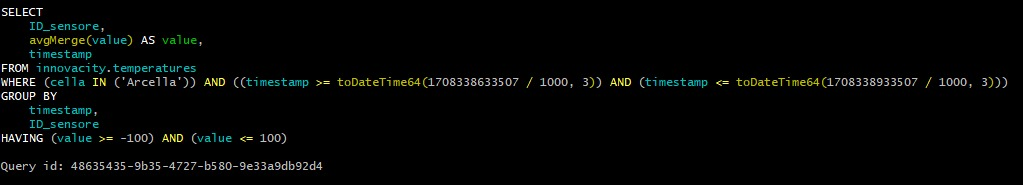
\includegraphics[width=1\textwidth]{../Images/SpecificaTecnica/ProjectionQuery.jpg}
        \caption{Query tipica - Grafana}
        \label{fig:ProjectionsQuery}
      \end{figure}
    senza l'utilizzo delle \textit{PROJECTIONS} il risultato è:
    \begin{figure}[H]
        \centering
        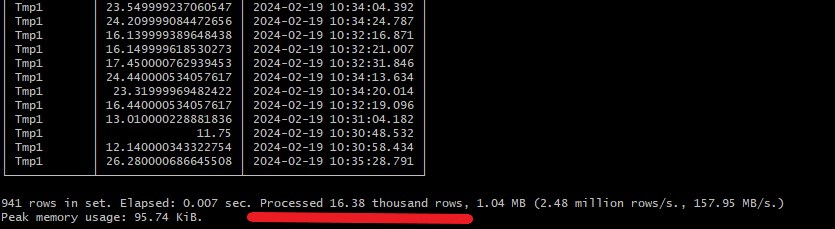
\includegraphics[width=0.9\textwidth]{../Images/SpecificaTecnica/SenzaProectionResult.jpg}
        \caption{Query tipica risultato senza projections}
        \label{fig:ProjectionsQueryWthout}
      \end{figure}
      ovvero sono state processate per ottenere il risultato della \textit{Query} \textbf{16,38 migliaia} di righe.

      Invece in seguito all'aggiunta delle \textit{PROJECTIONS}:
      \begin{figure}[H]
        \centering
        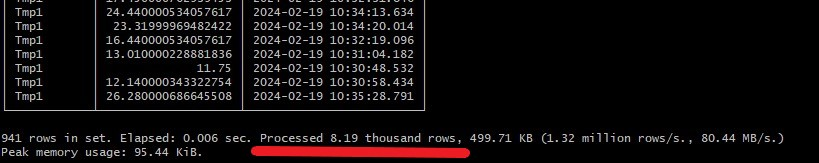
\includegraphics[width=0.9\textwidth]{../Images/SpecificaTecnica/ConProjectionRisultato.jpg}
        \caption{Query tipica risultato con projections}
        \label{fig:ProjectionsQueryWith}
      \end{figure}   
  ovvero sono state processate per ottenere il risultato della \textit{Query} \textbf{8,19 migliaia} di righe, circa la metà rispetto al risultato precedente consentendoci di apprezzare il miglioramento.
Inoltre tramite una \textit{Query} speciale è possibile visualizzare che la \textit{PROJECTIONS} è stata effettivamente utilizzata per ottenere il risultato della \textit{Query} in esame.
\begin{figure}[H]
    \centering
    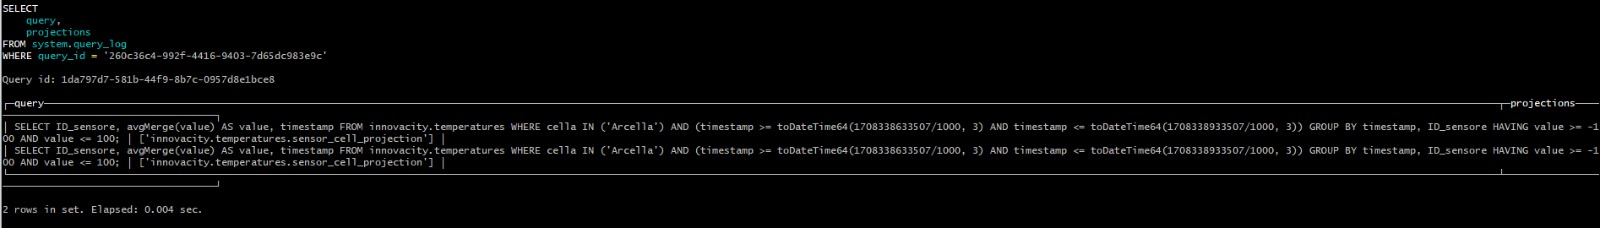
\includegraphics[width=1\textwidth]{../Images/SpecificaTecnica/ProjectionUsedByClickHouse.jpg}
    \caption{Uso della Projection}
    \label{fig:ProjectionsUsed}
\end{figure}

Prendendo in esempio un altra \textit{Query} fatta dall'applicativo dove viene effettuata la media globale di \textbf{170 mila }misurazioni di temperatura si possono apprezzare i benifiici dell'utilizzo delle \textit{PROJECTIONS} e alla fine dell'immagine anche il suo effettivo utilizzo per il calcolo del risultato.
Con l'utilizzo della \textit{PROJECTIONS} abbiamo:
\paragraph{Tabella: humidity\_kafka}
\begin{figure}[H]
    \centering
    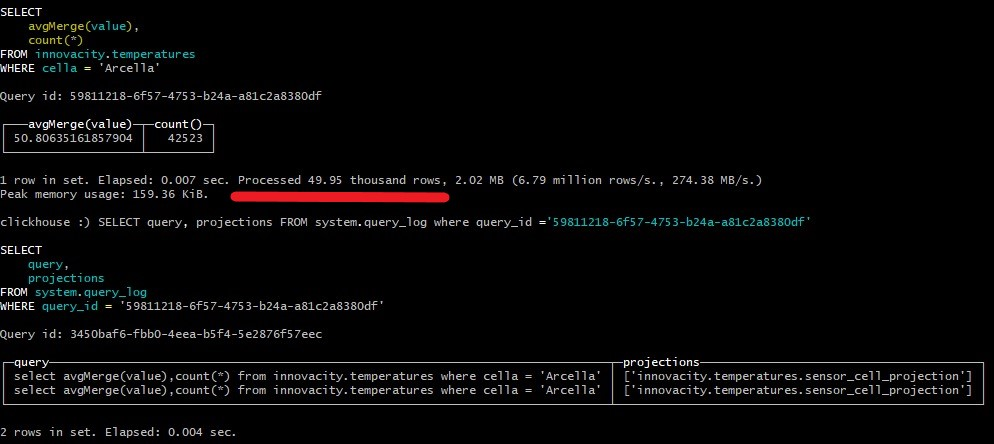
\includegraphics[width=1\textwidth]{../Images/SpecificaTecnica/query2ProjectionsWith.jpg}
    \caption{Query esempio Projection 2 - ClickHouse}
    \label{fig:with2proj}
  \end{figure}
Ovvero il totale di righe processate per ottenere il risultato è di \textbf{49,95 migliaia} con \textbf{0,07 secondi} di tempo utilizzati.
Si puo notare invece la differenza delle righe processate una volta rimossa la \textit{PROJECTIONS}:
\begin{figure}[H]
    \centering
    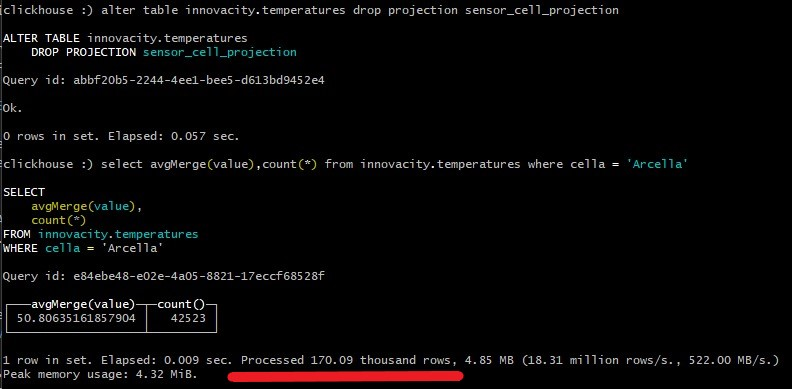
\includegraphics[width=1\textwidth]{../Images/SpecificaTecnica/query2ProjectionsWithout.jpg}
    \caption{Query esempio senza Projection 2 - ClickHouse}
    \label{fig:without2proj}
  \end{figure}

 Il totale di righe processate per ottenere il risultato è ora di \textbf{170,09 migliaia}, ovvero la totalità delle righe presenti nella tabella, con \textbf{0,09 secondi} di tempo utilizzati.

\subsubsection{Misurazioni umidità}
Le considerazioni relative al salvataggio delle misurazioni di umidità coincidono con quelle espresse nella sezione \ref{sec:tab_temperatures} riguardo alle misurazioni di temperatura.
\paragraph{Tabella: humidity\_kafka}
\begin{figure}[H]
    \centering
    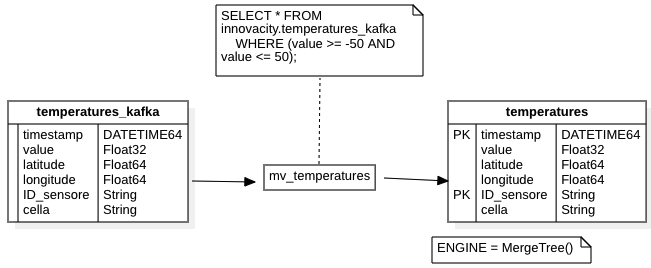
\includegraphics[width=1\textwidth]{../Images/SpecificaTecnica/temperatures.PNG}
    \caption{Tabella humidity\_kafka - ClickHouse}
    \label{fig:umidities_kafka}
  \end{figure}
Il dato della misurazione è di tipo Float32, l’equivalente di float nel linguaggio C. Il topic
kafka per ottenere i dati è: \textbf{humidity}.
\paragraph{Tabella: umidities}
\begin{figure}[H]
    \centering
    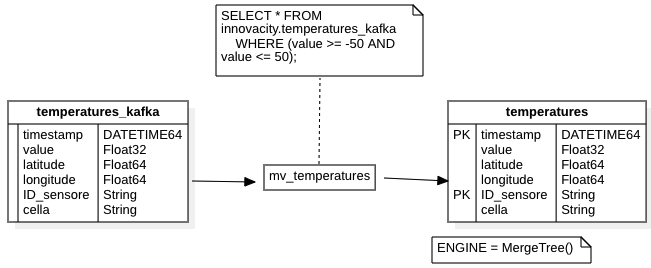
\includegraphics[width=1\textwidth]{../Images/SpecificaTecnica/temperatures.PNG}
    \caption{Tabella humidity - ClickHouse}
    \label{fig:umidities}
  \end{figure}

\paragraph{Projections per misurazioni di umidità} 
Date le stesse considerazioni fatte nella sezione: \ref{sec:temp_projections} anche per le misurazioni di umidità si è deciso di adottare le \textit{PROJECTION}.
I risultati dei benifiici perfettamente riconducibili a quelli per le misurazioni di temperatura alla sezione: \ref{sec:temp_projections_benefici}.

Di seguito vengono fornite le configurazioni delle proiezioni sulle tabelle delle misurazioni di umidità:

\begin{lstlisting}
    --Projection per tabella humidity
    ALTER TABLE innovacity.humidity ADD PROJECTION umd_sensor_cell_projection (SELECT * ORDER BY cella);
    ALTER TABLE innovacity.humidity MATERIALIZE PROJECTION umd_sensor_cell_projection;
\end{lstlisting}


\subsubsection{Misurazioni polveri sottili}Le considerazioni relative al salvataggio delle misurazioni di polveri sottili coincidono con quelle espresse nella sezione \ref{sec:tab_temperatures} riguardo alle misurazioni di temperatura.



\subsection{Grafana}
Grafana è un software open source per la visualizzazione e l'analisi dei dati. È progettato per funzionare con vari database di serie temporali, tra cui Clickhouse. Grafana offre un'interfaccia utente intuitiva e flessibile che consente di creare e condividere dashboard personalizzate per monitorare i dati in tempo reale. È ampiamente utilizzato per monitorare sistemi e applicazioni, nonché per analizzare e visualizzare dati in tempo reale.

\subsection{Dashboards}
Per soddisfare tutti i requisiti definiti in \textit{Analisi dei requisiti v2.0.0} sono state create due Dashboard:
\begin{itemize}
    \item \textbf{Dashboard Principale:} Questa dashboard fornisce una visualizzazione chiara e intuitiva delle misurazioni provenienti da tutti i sensori, di tutte le tipologie, distribuiti nell'area urbana. La dashboard include una mappa interattiva della città che mostra la posizione geografica di ciascun sensore e la relativa ultima misurazione. Inoltre, viene presentato il punteggio di salute della città o di celle specifiche.
    \item \textbf{Dashboard dedicata:} Mostra le misurazioni di una specifica tipologia di sensore selezionata dall'utente in modo più dettagliato e permette di effettuare le attività di filtraggio e aggregazione definite in \textit{Analisi dei requisiti v2.0.0}.
\end{itemize}




\subsubsection{ClickHouse data source plugin} \label{sec:click_plugin}
\paragraph{Documentazione:} \href{https://grafana.com/grafana/plugins/grafana-clickhouse-datasource/}{https://grafana.com/grafana/plugins/grafana-clickhouse-datasource/}

Questo plugin di grafana consente di connettersi a un'istanza di ClickHouse e di visualizzare i dati in tempo reale. È possibile eseguire query SQL personalizzate e visualizzare i risultati in forma di grafici, tabelle e pannelli personalizzati. Il plugin offre anche funzionalità di aggregazione e di calcolo dei dati, consentendo di analizzare e visualizzare i dati in modo flessibile e personalizzato.

\paragraph{Data sources configuration}
La configurazione del data source avviene tramite file \textit{yaml} che deve essere presente in \textit{"grafana/provisioning/datasources"}.
Il protocollo di trasporto utilizzato è TLS ma puo essere modificato nel file appena citato grazie al parametro di configurazione: "protocol".

\paragraph{Macro utilizzate}\label{sec:macros}
Per semplificare la sintassi e consentire operazioni dinamiche, come i filtri dell'intervallo di date, le queries al database Clickhouse possono contenere macro.
Quelle utilizzate sono:
\begin{itemize}
    \item \textbf{\$\_\_timeFilter(columnName)}: Permette di effettuare il filtro temporale alla query per ottenere le sole misurazioni all'interno dell'intervallo di tempo selezionato dall'utente.
    \item  \textbf{\$\_\_timeInterval(columnName)}: Permette di modificare il raggruppamento temporale delle misurazioni in automatico sulla base dell'ampiezza dell'intervallo temporale selezionato dall'utente.
    In questo modo è possibile avere una visione ottimizzate delle misurazioni.
\end{itemize}

\subsubsection{Variabili Grafana}
\paragraph*{Documentazione:} \href{https://grafana.com/docs/grafana/latest/dashboards/variables/}{https://grafana.com/docs/grafana/latest/dashboards/variables/}


 Le variabili in Grafana sono un potente strumento per rendere le dashboard dinamiche e interattive. Permettono di filtrare i dati visualizzati in base a valori scelti dall'utente, rendendo la dashboard più versatile e adattabile a differenti esigenze.
\paragraph*{Utilizzo delle variabili nella dashboard principale:}
Nella dashboard principale, le variabili sono:
\begin{itemize}
    \item \textbf{variabile \$cella}: per mostrare solo le misurazioni provenienti da determinate celle della città, 
    \item \textbf{variabili \$<TipoSensore>\_sensors\_id}: per mostrare le misurazioni di determinati sensori di un certo tipo.
\end{itemize}
Queste variabili all'interno delle query al database permettono il filtraggio delle misurazioni sulla base di quanto selezionato dall'utente.
Un esempio di query per la visualizzazione delle misurazioni time-series di temperatura è:
\begin{lstlisting}[style=code]
    SELECT    ID_sensore, avg(value) as value,
              $__timeInterval(timestamp) as timestamp
    FROM    innovacity.temperatures 
    WHERE    $__timeFilter(timestamp) AND cella IN ($Cella) AND ID_sensore in (${tmp_sensors_id})
    GROUP BY ID_sensore, timestamp;
\end{lstlisting}

La query esposta mostra anche l'utilizzo delle macro esposte in: \ref{sec:macros}
\paragraph*{Utilizzo delle variabili nella dashboard dedicata:}
Nella dashboard dedicata alla visualizzazione spefica delle misurazioni di una sola tipologia di sensori, le variabili sono:
\begin{itemize}
    \item \textbf{variabile \$cella}: per mostrare solo le misurazioni provenienti da determinate celle della città, 
    \item \textbf{variabili \$<TipoSensore>\_sensors\_id}: per mostrare le misurazioni di determinati sensori di un certo tipo.
    \item \textbf{variabili \$tabella}: per selezionare la tipoligia di sensore di cui si vuole visualizzare la dashboard dedicata e quindi la tabella del database da cui ricavare i dati.
    \item \textbf{\$aggregazione}: variabile per selezionare l'intervallo temporale di aggregazione delle misurazioni
    (Automatico, Secondo,Minuto,Ora,Giorno,Mese,Nessuno).
    Nel caso della selezione della modalità "Automatico" si utilizzza l'intervallo temporale di aggregazione più opportuno sulla base dell'ampiezza dell'intervallo temporale selezionato dall'utente.
    \item \textbf{\$Max\_value}: variabile ad input numerico per filtrare le misurazioni con valore al di sotto di quello indicato.
    \item \textbf{\$Min\_value}: variabile ad input numerico per filtrare le misurazioni con valore al di sopra di quello indicato.
\end{itemize}
\paragraph{Variable Panel plugin}
\textbf{Documentazione:} \href{https://volkovlabs.io/plugins/volkovlabs-variable-panel/}{https://volkovlabs.io/plugins/volkovlabs-variable-panel/}
Il plugin permette di creare dei pannelli grafana che possono essere posizionati ovunque nella Dashboard e che consentono di selezionare i valori delle variabili.
Inoltre permette la visualizzazione ad albero delle variabili utile nel nostro caso dove i sensori sono contenuti all'interno di celle della città.

\subsubsection{Grafana alerts}
\textbf{Documentazione}\href{https://grafana.com/docs/grafana/latest/alerting/}{https://grafana.com/docs/grafana/latest/alerting/}


Grafana offre un sistema di alerting completo per monitorare i dati e inviare notifiche quando si verificano determinate condizioni. Le notifiche possono essere inviate tramite diversi canali, tra cui email, Slack, Telegram e Discord.

\paragraph{Alert Rule}
Per poter configurare un alert è necessario creare una regola di alert. La regola di alert viene impostata tramite query al data source e fa scattare l'alert quando la query restituisce un risultato che soddisfa le condizioni impostate.
Gli alert impostati sono per:
\begin{itemize}
    \item Quando un sensore di temperatura registra una temperatura superiore ai 40°C;
    \item Quando un sensore di polveri sottili supera i 50 microgrammi al metro cubo;
    \item Quando un sensore di guasti elettrici rileva un guasto.
\end{itemize}

Gli alert attraversano 3 stati:
\begin{itemize}
    \item \textbf{Pending:} indica che un alert è stato attivato, ma la sua valutazione non è ancora stata completata.
                            Quando si è in questo stato è perchè il valore della query di alert è stato valutato e risulta essere vero ma la configurazione della regola di allerta ha impostato che l'allerta deve essere attiva per un certo periodo di tempo prima di essere considerata vera e quindi inviare la notifica.
\item \textbf{Firing:}  indica che un alert è stato attivato e la sua valutazione ha confermato che la condizione di alert è soddisfatta per il periodo impostato nella regola e quindi viene inviata la notifica ai canali impostati.
\item \textbf{OK:} indica che un alert è stato disattivato e la sua valutazione ha confermato che la condizione di alert non è più soddisfatta.

Le regole di allerta sono impostabili tramite l'interfaccia grafica di Grafana e vengono esportate in formato \textit{yaml} ed inserite in "/provisioning/alerting".
                            
\end{itemize}

\paragraph{Configurazione il canale di notifica}
Per configurare i canali di notifica è necessario andare in "Alerting" e selezionare "Notification channels" dall'interfaccia grafica di Grafana.

Per il progetto è stato scelto Discord come unico canale di notifica.
Per configurare il canale di notifica è necessario:
\begin{itemize}
    \item Seleziona Discord come canale di notifica.
    \item Inserisci il webhook URL del tuo canale Discord.
    \item Personalizza il messaggio di notifica.
\end{itemize}

Anche le impostazioni di configurazione del canale di notifica sono esportabili in formato \textit{yaml} e vengono inserite in "/provisioning/alerting".

\paragraph{Notification policies}
Le norme di notifica negli Alert di Grafana sono un modo potente per gestire l'invio degli alert a diversi canali di notifica.

Per una spiegazione dettagliata della configurazione si rimanda alla documentazione ufficiale di Grafana: \href{https://grafana.com/docs/grafana/latest/alerting/alerting-rules/create-notification-policy/}{https://grafana.com/docs/grafana/latest/alerting/alerting-rules/create-notification-policy/}

Anche le impostazioni delle notification policies sono esportabili in formato \textit{yaml} e vengono inserite in "/provisioning/alerting".

\subsubsection{Altri plugin utilizzati}
\paragraph{Orchestra Cities Map plugin}
\textbf{Documentazione:} \href{https://grafana.com/grafana/plugins/orchestracities-map-panel/}{https://grafana.com/grafana/plugins/orchestracities-map-panel/}

Il plugin Orchestra Cities Map per Grafana estende il pannello Geomap di Grafana con diverse funzionalità avanzate per la visualizzazione di dati geolocalizzati su mappe:

Funzionalità principali:
\begin{itemize}
    \item \textbf{Supporto per GeoJSON}: Permette di visualizzare dati geoJSON su mappe, come shapefile di città, regioni o stati.
    \item \textbf{Icone personalizzate}: Puoi utilizzare icone personalizzate per rappresentare diversi tipi di dati sui punti mappa.
    \item \textbf{Popup informativi}: Mostra popup con informazioni dettagliate quando si clicca su un punto mappa.
    \item \textbf{Strati multipli}: Permette di creare più strati sovrapposti per visualizzare diversi set di dati sulla stessa mappa.
    \item \textbf{Filtraggio e ricerca}: Puoi filtrare i punti mappa in base a diversi criteri, come proprietà dei dati o valori delle metriche.
    \item \textbf{Colorazione dei punti}: Puoi colorare i punti mappa in base a valori di metriche o ad altri criteri.
    \item \textbf{Legende personalizzate}: Puoi creare legende personalizzate per spiegare il significato dei colori e delle icone utilizzati nella mappa.
\end{itemize}

Viene utilizzato per poter visualizzare in modo diverse le icone dei diversi tipi di sensori dislocati nella città oltre che l'ultima misurazione effettuata ovvero lo stato attuale del sensore.
